%%%%%%%%%%%%%%%%%%%%%%%%%%%%%%  IEEEsample.tex
%%%%%%%%%%%%%%%%%%%%%%%%%%%%%%%%%%%%%%%%%
%%%%%%%%%%%%%%%%%%%%%%%    More information: see the header of IEEEtran.sty
%%%%%%%%%%%%%%%%%%%%%%%
%%%%%%%%%%%%%%%%%%%%%%%%%%%%%%%%%%%%%%%%%%%%%%%%%%%%%%%%%%%%%%%%%%%%%%%%%%%%%%%%
%%%%

\documentclass[10pt,twocolumn]{IEEEtran}
%\documentclass[conference]{IEEEtran}

%%%\IEEEoverridecommandlockouts


%% set page size to US letter
\special{papersize=8.5in,11in}
\setlength{\pdfpageheight}{\paperheight}
\setlength{\pdfpagewidth}{\paperwidth}

\usepackage{xspace}
%\newcommand{\Grobner}{Gr\"{o}bner\xspace}

\usepackage{algorithm}
\usepackage[noend]{algpseudocode}
\renewcommand{\algorithmicrequire}{\textbf{Inputs:}}
\renewcommand{\algorithmicensure}{\textbf{Outputs:}}



%% \usepackage[vlined,boxed,ruled]{algorithm2e}
%% %%for algorithm2e package, label has to be following caption in the same line!!!
%% \renewcommand{\algorithmcfname}{ALGORITHM}
%%  \SetAlFnt{\small}
%%  \SetAlCapFnt{\small}
%%  \SetAlCapNameFnt{\small}
%%  \SetAlCapHSkip{0pt}
%%  \IncMargin{-\parindent}

%% %% \RequirePackage{times}
%%  \RequirePackage{algorithmic}
%%  \PassOptionsToPackage{boxed}{algorithm}
%%  \RequirePackage{algorithm}
%%  \RequirePackage{multicol}
 \DeclareMathAlphabet{\mathtsl}{OT1}{ptm}{m}{sl}

%\def\BibTeX{{\rm B\kern-.05em{\sc i\kern-.025em b}\kern-.08em1
%    T\kern-.1667em\lower.7ex\hbox{E}\kern-.125emX}}

%\newtheorem{theorem}{Theorem}
%\newtheorem{lemma}{Lemma}
%\newtheorem{example}{Example}
%\newtheorem{corollary}{Corollary}

\RequirePackage{amssymb, mathptm}
\usepackage{amsbsy}
\usepackage{amsthm}
\usepackage{graphicx}
\usepackage{helvet}
\usepackage{enumerate}
\usepackage{amsmath}
\usepackage{amsfonts}
\usepackage{graphicx}
\usepackage{multirow}
\usepackage{subfig}
\usepackage{comment}
\usepackage{cases}
\usepackage{xcolor}
\usepackage{epstopdf}
\usepackage[normalem]{ulem}
\usepackage{hhline}
%%indent in algorithm


%\setcounter{page}{1}


% New command for the table notes.
\def\tabnote#1{{\small{#1}}}

% New command for the line spacing.
\newcommand{\ls}[1]
    {\dimen0=\fontdimen6\the\font
     \lineskip=#1\dimen0
     \advance\lineskip.5\fontdimen5\the\font
     \advance\lineskip-\dimen0
     \lineskiplimit=.9\lineskip
     \baselineskip=\lineskip
     \advance\baselineskip\dimen0
     \normallineskip\lineskip
     \normallineskiplimit\lineskiplimit
     \normalbaselineskip\baselineskip
     \ignorespaces
    }
%\renewcommand{\algorithmicrequire}{\textbf{Input:}}
%\renewcommand{\algorithmicensure}{\textbf{Output:}}

\newcommand{\beq}{\begin{equation}}
\newcommand{\eeq}{\end{equation}}
\newcommand{\beqarr}{\begin{eqnarray}}
\newcommand{\eeqarr}{\end{eqnarray}}
%\newcommand{\ov}{\overline}
\newcommand{\ov}{\bar}
\newcommand{\xor}{\bigoplus}
\newcommand{\Fm}{{\mathbb{F}}}
\newcommand{\myfontsize}{\fontsize{7}{9}\selectfont}


%the following is for space before and after align or other equation environment.

%%
\newtheorem{Algorithm}{Algorithm}[section]
\newtheorem{Definition}{Definition}[section]
\newtheorem{Example}{Example}[section]
\newtheorem{Proposition}{Proposition}[section]
\newtheorem{Lemma}{Lemma}[section]
\newtheorem{Theorem}{Theorem}[section]
\newtheorem{Corollary}{Corollary}[section]
\newtheorem{Conjecture}{Conjecture}[section]
\newtheorem{Problem}{Problem}[section]
\newtheorem{Notation}{Notation}[section]
\newtheorem{Setup}{Problem Setup}[section]

%%%

%%set spacing between table columns
\setlength{\tabcolsep}{3pt}

\begin{document}

%\thispagestyle{empty}
%\pagestyle{empty}

%\ls{1.5}


\title{\Large\textsc{Boolean Gr\"obner Basis Reductions on \textcolor{red}{Finite Field} Datapath Circuits using the Unate Cube Set Algebra}}
\author{Utkarsh Gupta, Priyank Kalla, {\it Senior Member, IEEE}, Vikas Rao 
%Electrical \& Computer Engineering, University of Utah \vspace{-0.2in}
\thanks{This work has been supported in part by grants from the US
  National Science Foundation CCF-1320335 and CCF-1619370. The authors
are with the Electrical \& Computer Engineering Department at the
University of Utah in Salt Lake City, USA. Contact author: Priyank
Kalla (kalla@ece.utah.edu).  }
}
%\affiliation{Electrical \& Computer Engineering, University of Utah}
% \email{}    
 
 
\maketitle
\thispagestyle{empty}
% Modified by  K. Kobayashi \maketitle 

%\markboth{MS Proposal by Tim Pruss}{}
\newcommand{\Fq}{{\mathbb{F}}_{q}}
\newcommand{\Fkk}{{\mathbb{F}}_{2^k}}
\newcommand{\Zkk}{{\mathbb{Z}}_{2^k}}
\newcommand{\Ftwo}{{\mathbb{F}}_{2}}
\newcommand{\Fkkx}[1][x]{\ensuremath{\mathbb{F}}_{2^k}[#1]\xspace}
\newcommand{\Grobner}{Gr\"{o}bner\xspace}
\newcommand{\B}{{\mathbb{B}}}
\newcommand{\Z}{{\mathbb{Z}}}
\newcommand{\F}{{\mathbb{F}}}
\newcommand{\G}{{\mathcal{G}}}
\newcommand{\alert}[1]{\textcolor{red}{#1}}

\newcommand{\spec}{{\it Spec}\xspace\ \xspace}
%%%

\newcommand{\debug}[1]{\textcolor{red}{[ #1 ]}}


%%%%%%%%%%%%%%%%%%%% Include your files here %%%%%%%%%%%%%%%%%%%%%
\begin{abstract}
Recent developments in formal datapath verification make efficient use 
of symbolic computer algebra algorithms for formal verification. The
circuit is modeled as a set of polynomials over Boolean (or
pseudo-Boolean) rings, and  Gr\"obner basis (GB) reductions are
performed over these polynomials to derive a canonical
representation. GB reductions of Boolean polynomials tend to cause
intermediate expression swell (term explosion problem) -- often making
the approach infeasible in a practical setting. To overcome these
problems,  this paper describes a logic synthesis analogue of GB
reductions over Boolean polynomials, using the unate cube set algebra
over characteristic sets. By representing Boolean polynomials as
characteristic sets using Zero-suppressed BDDs (ZBDDs), implicit
algorithms can be efficiently designed for GB-reduction on digital
circuits. We show that imposition of circuit-topology based monomial
orders on ZBDDs enables an implicit implementation of polynomial
division, canceling multiple monomials in one-step. 
%Other recent
%strategies of GB-reduction on circuits can also be implemented
%efficiently on ZBDDs. 
Experiments performed over various finite field
arithmetic architectures demonstrate the efficiency of our 
algorithms and implementations as compared to conventional explicit
methods. 
\end{abstract}

\section{Introduction}

Automated formal verification and equivalence checking of arithmetic
datapath circuits is challenging. Conventional verification
techniques, such as those based on binary  decision diagrams (BDDs)
\cite{BRYA86}, And-Invert-Graph (AIG) based reductions with SAT or
SMT-solvers \cite{alanmi:cec:iccad2006}, etc., are infeasible in
verifying complex datapath designs. Such designs often implement
algebraic computations over bit-vector operands, therefore finite
integer rings \cite{wienand:cav08} \cite{wedler:date11} or finite
fields \cite{lv:tcad2013} \cite{pruss:tcad}
are considered appropriate models to devise decision
procedures for verification. For this reason, the verification
community has explored the use of algebraic geometry and symbolic
algebra algorithms for verification. 


In such a setting, the logic gates of the circuit are modeled by way
of a set of multivariate polynomials $F=\{f_1,\dots,f_s\}$ in rings
$R[x_1,\dots,x_n]$. Usually, the coefficients $R = \Z, \Zkk,$ or $\Fkk$,
depending on whether the integer, finite integer ring
$\pmod{2^k}$, or respectively the finite field (of $2^k$ elements)
model is employed for verification. This set of polynomials $F$
generates an ideal, and for verification it is required to compute a
{\it \Grobner basis (GB)} \cite{gb_book} of this ideal. Reducing the
primary \textcolor{red}{output polynomials} of the circuit modulo this
GB  results in a unique canonical polynomial expression, and it can be
used for equivalence checking.  


The GB problem exhibits high computational complexity. 
Indeed, computing a GB (using Buchberger's \cite{buchberger_thesis} or
the $F_4$ algorithm \cite{f4}) for large circuits is practically
infeasible. Managing this complexity ought to be a major goal of any
approach. 

\subsubsection{State-of-the-art \& Limitations} Recent
approaches \cite{wienand:cav08} \cite{lv:tcad2013} have discovered that
particularly for circuit verification problems, the
expensive GB computation can be avoided altogether. For arbitrary
combinational \cite{wienand:cav08} \cite{lv:tcad2013} and sequential
circuits \cite{xiaojun:hldvt2016}, a specialized term order 
$>$ can be derived by analyzing the topology of the given 
circuit. This term order is derived by performing a reverse
topological traversal of the circuit, and in this manuscript we refer 
to it as the {\it Reverse Topological Term Order} (RTTO). 
Imposition of RTTO $>$ on the polynomial ring
{\it renders the set of polynomials of the circuit itself a
GB.} Subsequently, the verification problems can be solved solely by
way of GB-reduction (using multi-variate polynomial division), without
any need to explicitly compute a GB. It has now become standard
practice to make use of RTTO-style term orders to solve various formal 
verification problems on digital circuits 
(see for example
\cite{wienand:cav08,lv:tcad2013,wedler:date11,ciesielski:dac2015,farimah:micro2015,rolf:date16}), 
where the early techniques of \cite{wienand:cav08} \cite{lv:tcad2013}
have been extended and improved to verify integer and floating point
arithmetic circuits \cite{ciesielski:dac2015,rolf:date16,rolf:fmcad17}. 


%% For instance,
%% \cite{ciesielski:dac2015} and \cite{rolf:date16} get more insights
%% from the circuit structure that  dictate specific rules on the order of
%% polynomials chosen in GB-reduction -- by accounting for topological
%% levels, reconvergent fanouts, AND-XOR gates with common inputs,
%% etc. 

A common theme among all these relevant works is that {\it by virtue
of RTTO, they move the complexity of verification from one of
computing a GB to that of GB-reduction by way of multivariate
polynomial division.} Moreover, since the \Grobner basis is derived
from the logic gates of the circuit, {\it it comprises Boolean
polynomials.} \textcolor{red}{Boolean polynomials (formally defined in
  Section \ref{sec:prelim})  consist of terms that have coefficients
  from $\Ftwo = \{0,1\}$, and monomials that are a product of
  variables where the degree of each variable is also restricted to
  the set $\{0,1\}$.} For example, in the verification of finite field 
circuits, the overall problem is modeled over the ring
$\Fkk[x_1,\dots,x_n]$; and %, where $\Fkk$ is the field of $2^k$ elements. 
since $\Fkk \supset \Ftwo$, the approaches incorporate computations
over many Boolean polynomials. Similarly, the techniques of
\cite{wedler:date11} use a pseudo-Boolean polynomial model which also
encompasses computations $\pmod{x^2=x}$. \textcolor{red}{Pseudo-Boolean
  polynomials %(defined later    in Section \ref{sec:prelim}) 
are those that have coefficients in integers, and monomials are a
product of variables, where the degree of each variable is still
restricted to the set $\{0,1\}$.}  The aforementioned approaches will
benefit greatly by a {\it dedicated,  
domain-specific implementation of GB-reduction w.r.t. Boolean polynomials,
carried out on the given circuit under RTTO $>$}. So far, the above
techniques  
\cite{wienand:cav08,pruss:tcad,lv:tcad2013,rolf:date16,ciesielski:dac2015,cunxi:aspdac17}
use a general-purpose polynomial division approach, together with an
explicit representation, for this GB-reduction. 
%While some of these
%approaches %\cite{ciesielski:dac2015,rolf:date16} 
%do perform the reduction in some specific ways -- e.g., mimicking
%GB-reduction under RTTO $>$ by substitution \cite{rolf:date16}, or using
%TEDs to perform input-output signature comparisons \cite{ciesielski:dac2015},
%or the use of $F_4$-style GB-reduction on a coefficient matrix
%\cite{lv:tcad2013} -- 
Moreover, the overall concept of polynomial division is
still utilized in its rudimentary form, involving iterative
cancellation of monomials ``1-step at a time'' on explicit
data-structures. Despite recent efforts, such GB-reductions can lead
to {\it a worst-case size explosion problem}, which needs to be
addressed. 


\subsubsection{Objective \& Rationale} This paper addresses the
problem of deriving canonical representations for datapath circuits
as Boolean polynomials. These canonical Boolean polynomials are
used for equivalence checking of datapath designs. The canonical
representation requires a \Grobner basis reduction modulo a set of
Boolean polynomials. 
%This reduction can result in space and time
%explosion and make verification infeasible. 
To make this GB-reduction
on circuits more efficient, this paper describes new techniques,
algorithms and implementations, specifically targeted for 
circuit verification under RTTO $>$.  We make use of
the {\it implicit} characteristic set representation for storing and
manipulating Boolean polynomials using {\it Zero-Suppressed BDDs
(ZBDDs)} \cite{zbdd}. By analyzing the {structure of ZBDDs} for 
polynomial representation under RTTO $>$, we show how this 
GB-reduction can be efficiently implemented using algorithms that
specifically manipulate the ZBDD graph, by interpreting Boolean
polynomial manipulation as the {\it algebra of unate cube sets.}

The algebraic objects
used to model the polynomial ideals derived from digital circuits are
rings of Boolean polynomials.
%generally of two types: (i) multi-variate polynomial
%rings with coefficients from the finite fields ($\Fkk$) of $2^k$
%elements, i.e. $\Fkk[x_1, \dots, x_n]$; and (ii)  quotient rings of the
%type $\Zkk[x_1, \dots, x_n] \pmod{ \langle x_i^2 - x_i\rangle}$
%corresponding to the pseudo-Boolean function models; here 
%$\Zkk = \Z \pmod{ 2^k}$. Over circuits, both models incorporate
%computations over {\it Boolean   polynomials}: (i) $\Ftwo (\equiv \B)
%\subset \Fkk$; whereas (ii) also encompasses (pseudo-) Boolean
%computations $\pmod{ x^2 = x}$.
%; \cite{wienand:cav08} refer to it as ``arithmetic bit-level''. 
When Boolean functions are represented in $\F_2$ (AND/XOR
expressions), and that too as a canonical \Grobner basis, the
representation tends to explode. 
%(depicted later in Section \ref{sec:motiv}).  
Polynomial representations employed in computer
algebra tools, such as the {\it dense-distributive 
data-structure} of the {\sc Singular} computer algebra tool
\cite{DGPS}, are inefficient for this purpose. Since addition and
multiplication $\pmod{2}$ are equivalent to XOR and AND operations,
respectively, GB-reduction can be viewed as a polynomial analog of a
specialized {\it AND/XOR Boolean decomposition} problem. Moreover,
the monomials of a Boolean polynomial are a product of literals in
positive polarity, which can be viewed as {\it unate cubes} in logic
synthesis. Clearly, implicit Boolean set representations such as
decision diagrams could be employed for \Grobner basis reductions over
Boolean polynomials. 
%The decision diagram of choice here is the ZBDD,
%\cite{zbdd}, 
%because of its power to represent and manipulate sparse
%combinatorial problems -- particularly ``sets of combinations'' --
%using the unate cube set algebra framework \cite{zbdd_unate}.  
%Monomials of a Boolean polynomial can be
%interpreted as {\it unate cubes} -- i.e. products of literals in
%positive polarity. Each cube represents one combination, and each
%literal represents an object chosen in the combination. Thus,
%GB-reduction on circuits resembles a classical logic synthesis
%problem, justifying the use of ZBDDs.


\subsubsection{Technical Contributions} %First and foremost, 
%% We address the problem of \Grobner basis reductions over Boolean
%% polynomials to derive canonical representations for the functions
%% implemented by datapath circuits. Our approach makes use of 


%% For this we present new algorithms and

We first describe when and how the GB-reduction encounters a
term-explosion (exponential blow-up) under RTTO $>$, which cannot be
easily overcome by explicit representations. We show that ZBDDs can
avoid this exponential blow-up -- thereby justifying their use. We
describe how Boolean polynomials can be represented using ZBDDs under
the special term ordering constraint imposed due to RTTO $>$. The
implementation of classical polynomial division algorithms that
iteratively cancel one monomial in every step is described on ZBDDs.
Subsequently, {\it we show that RTTO $>$ imposes 
a special structure on ZBDDs that allows to implement reduction
techniques that implicitly cancel multiple   monomials in every step
of polynomial division}. Moreover, due to RTTO $>$,  the
subexpressions that are required for polynomial division are also
readily available as subgraphs in the ZBDDs. Our algorithm exploits
this special structure, thus improving GB-reduction in both space and
time. 
%Moreover, we also implement the specialized
%GB-reduction approach of \cite{rolf:date16} using our ZBDD
%framework. 

Using an implementation integrated with the CUDD \cite{cudd} package,
we perform extensive experiments on datapath circuits for deriving the
canonical representation of the functions implemented by them. The
benchmark designs include various cryptography primitives, such as
finite field multipliers, elliptic curve point addition circuits, and
also  sequential finite field circuits. Experiments conducted on these
benchmarks show {\it orders of magnitude improvement} using our
implementation of GB-reduction, as compared against contemporary
methods. In fact, for these benchmarks, our bit-level (Boolean)
approach is much faster than the word-level approaches
(e.g. \cite{pruss:tcad}). 

We also describe the limitations of our approach when it is
applied to integer arithmetic circuits. We analyze these limitations
and show that for integer arithmetic circuits, a word-level symbolic
reasoning engine is needed to control the monomial explosion
problem. This is not a limitation of our 
algorithms, but rather of the bit-level model in verifying integer
arithmetic circuits. Finally, we are not concerned with equivalence
checking of random logic circuits; AIG-based reductions for
SAT-based verification techniques \cite{alanmi:cec:iccad2006} are more
suitable and efficient for such applications. 



\subsubsection{Paper Organization} The following section reviews
relevant previous work on \Grobner basis based verification of
datapath circuits, and the literature on Boolean \Grobner basis and
applications. Section \ref{sec:prelim} describes the mathematical
background on \Grobner basis reductions, the RTTO based term order
$>$, and how these concepts are applied to datapath
verification. Section \ref{sec:unate} motivates how and why the
Boolean GB-reduction can be viewed as the unate cube set
algebra. Section \ref{sec:theory} describes the theory, algorithms and
implementations for GB-reduction for Boolean polynomials using
ZBDDs. Section \ref{sec:exp} describes the experiments conducted for
verification using our approach, and Sec \ref{sec:conc} concludes the
paper. 


\section{Related Previous Work}
\label{sec:prev}

In the past decade, computer algebra and algebraic geometry based
datapath verification has received a lot of attention, where the
verification problems are formulated in terms of ideal membership,
canonical GB-reductions, or projections of
varieties. The work of \cite{iccad05} used a GB-reduction
approach to derive canonical representations of (word-level) RTL
datapath descriptions over finite rings $\Zkk$. Using the same finite
ring model, \cite{wienand:cav08} addressed data correctness properties
of arithmetic bit-level implementations using a \Grobner basis
formulation. This paper showed how an efficient term order $>$
can be derived from the circuit to simplify the computation. 


In
\cite{lv:date2012} and \cite{lv:tcad2013}, the authors addressed formal
verification of finite field arithmetic circuits using the Strong
Nullstellensatz formulation over $\Fkk$. Using a set ($F$) of
polynomials to describe the logic circuit, along with a set of
vanishing polynomials ($F_0$) over the field $\Fkk$, the verification
problem was formulated as a (radical) ideal membership test, requiring 
a \Grobner basis. Drawing inspirations from \cite{wienand:cav08},
the authors in \cite{lv:date2012} also exploited the same concept of deriving a
specialized term order $>$ to simplify the ideal membership test. In
particular, it was shown that $>$ could be derived by performing a
{\it reverse topological traversal} on the circuit. Imposition of this
term order $>$ rendered the set of polynomials $F\cup F_0$ itself a
\Grobner basis, and verification was then performed simply by a
GB-reduction. This GB-reduction was 
subsequently formulated as Gaussian elimination on a coefficient
matrix \cite{lv:tcad2013,pruss:tcad} in the style of the $F_4$
algorithm; called $F_4$-style reduction in the sequel. 

Formulations of a similar flavor (GB-reduction under the
specialized term order $>$ derived from the circuit) were used
and integrated with SMT-solvers \cite{wedler:date11} for verification
using a pseudo-Boolean model (akin to $\Zkk[X] \pmod{X^2-X}$). More
recently, these concepts have been applied to verify integer
arithmetic \cite{ciesielski:dac2015,rolf:date16}, and also floating
point circuits \cite{rolf:fmcad17}. The authors
in~\cite{cunxi:aspdac17} show that the reduction process can be
{\it parallelized} by performing reduction for each output bit
independently.   

%The above approaches exploit the
%structure of the circuit to derive a term order $>$ that simplifies
%verification to a (set of) \Grobner basis reductions, of which
Polynomial division algorithms form the core computation in the above
techniques. Almost all of the 
aforementioned techniques use a classical polynomial division
approach. While some of these approaches
%\cite{ciesielski:dac2015,rolf:date16}  
do perform the reduction in 
some specific ways -- e.g., mimicking GB-reduction under RTTO $>$ by
substitution \cite{rolf:date16}, or using TEDs to perform input-output
signature comparisons \cite{ciesielski:flow}, or the use of
$F_4$-style GB-reduction on a coefficient matrix
\cite{lv:tcad2013,pruss:tcad} --  the overall concept of polynomial
division is still utilized in its rudimentary form, involving
iterative cancellation of monomials ``1-step at a time'' on explicit
data-structures. 
%In contrast, this paper improves the \Grobner basis
%reduction under RTTO $>$ using an implicit data-structure and
%algorithms that cancel multiple monomials 


\subsection{Boolean \Grobner Basis} 
The symbolic algebra community 
has studied properties of Boolean \Grobner bases 
\cite{michon:bool-ring2006} \cite{polybori:2009}. Boolean GB
formulations have also been used for SAT solving \cite{CEI:stoc-96},
e.g. to derive proof refutation, and for  model checking
\cite{Avrunin:CAV} \cite{vardi-iasted07}. From among these, the work
of PolyBori \cite{polybori:2009} comes closest to ours, and is a
source of inspiration for this work. PolyBori proposed the use of
ZBDDs to compute Gr\"obner bases for Boolean polynomials. PolyBori is
a {\it generic} Boolean GB computational engine that caters to many
permissible term orders. Its division algorithm is also generally
based on the conventional concept of canceling one monomial in every
step of reduction. In contrast, our algorithms are tailored for
GB-reduction under the RTTO $>$. The efficiency of our approach stems
from the observation that the RTTO $>$ imposes a special structure on
the ZBDDs, which allows for multiple monomials to be canceled in one
division-step, along with simplifying the search for
divisors. Experiments show that our approach is an order of magnitude
faster than PolyBori. 


%% \underline{\it Paper Organization:} The following section describes
%% our notation and preliminary concepts. Section \ref{sec:limit}
%% describes the limitations of contemporary approaches and shows how
%% ZBDDs may overcome these. Section \ref{sec:alg} describes our
%% algorithms and implementations of GB-reduction on ZBDDs w.r.t the RTTO
%% $>$. Section \ref{sec:integer} describes how the recent methodologies
%% for integer multiplier circuits can be implemented and improved
%% computationally using ZBDDs. Experiments are described in Section
%% \ref{sec:exp}. Section \ref{sec:concl} concludes the paper. 

%\section{Preliminaries: Notation and Background}
\section{Background: \Grobner Basis Reduction and Canonical Representations}
\label{sec:prelim}

%This section provides a brief description of the fundamental concepts of: 
%%i) commutative algebra including polynomial rings, polynomial division, ideals, 
% Gr\"obner basis and their application in verification of circuits;
%ii) the algebra of unate cube sets; and iii) the use of ZBDDs as an
%implicit set representation for manipulation of Boolean polynomials.

%\subsection{Computer Algebra}

% i.e., $G = GB(J) \Leftrightarrow\  \forall f \in J : f \neq 0 \ \exists g_i \in G :
%lm(g_i)\mid lm(f)$. 

\par Let $\B =\{0,1\}$ denote the Boolean domain, $\F_2$ the finite field
of 2 elements ($\B \equiv \F_2$), and $R = \F_2[x_1, \dots, x_n]$
the  polynomial ring over variables $x_1, \dots, x_n$ with
coefficients in $\F_2$.  
%Since $\Fkk$ is a $k$-dimensional extension of $\F_2$, we
%have that $\Fkk \supset \F_2$ and all $\Fkk (k \geq 1)$ are of
%characteristic 2. 
Operations in $\F_2$ are performed $\pmod{ 2}$, so $-1=+1$ in
$\F_2$. We will use $+ ,\cdot$ to denote addition and multiplication in
$R$, and $\neg, \vee, \wedge$ and $\oplus$ to denote Boolean negation,
OR, AND and XOR operations, respectively. 

A polynomial $f \in R$ is written as a finite sum of terms 
$f = c_1 X_1 +  c_2 X_2 + \dots + c_t X_t$.  Here $c_1, \dots, c_t$
are coefficients and $X_1, \dots, X_t$ are monomials, i.e. power
products of the type $x_1^{e_{1}}\cdot x_2^{e_{2}}\cdots x_n^{e_{n}}$, 
$e_i \in \Z_{\geq  0}$. To systematically manipulate the
polynomials, a monomial order $>$ (also called a term order) is
imposed on the ring. This order $>$ is a total order and a well
order on all the monomials of $R$ such that multiplication by a
monomial preserves the order\footnote{Lexicographic ({\it lex}) and
  degree-lexicographic ({\it deglex}) are examples of such permissible
  monomial orders.}. All polynomials in $R$ are represented using
$>$. Subject to $>$, when a polynomial is written as 
$f = c_1 X_1 +  c_2 X_2 + \dots + c_t X_t$ 
 such that  $X_1 >X_2 > \dots >  X_t$, we call  $lt(f) = c_1 X_1,
 ~lm(f) = X_1, ~lc(f) = c_1$, the {\it leading   term}, {\it   leading
   monomial} and {\it   leading coefficient} of $f$,
 respectively, with $lt(f) = lc(f)\cdot lm(f)$. 
We also denote tail($f$) = $f - lt(f) = c_2X_2 + \dots + c_t X_t$. 
In this work, we are mostly concerned with terms ordered
lexicographically ({\it lex}). 

\begin{Definition} [Boolean Polynomial]
Let $f = c_1 X_1 + \dots + c_t X_t$ be a polynomial in
$\F_2[x_1,\dots,x_n]$ such that the coefficients $c_i \in \{0, 1\}$,
and monomials $X = x_1^{e_{1}}\cdot x_2^{e_{2}}\cdots x_n^{e_{n}}, e_i
\in \{0,1\}$. 
Then $f$ is called a {\bf Boolean polynomial}. For Boolean polynomials
$lt(f) = lm(f)$. 
\end{Definition}

\textcolor{red}{\begin{Definition} [Pseudo-Boolean Polynomial]
Let $f = c_1 X_1 + \dots + c_t X_t$ be a polynomial
such that the coefficients $c_i \in \mathbb{Z}$,
and monomials $X = x_1^{e_{1}}\cdot x_2^{e_{2}}\cdots x_n^{e_{n}}, e_i
\in \{0,1\}$. 
Then $f$ is called a {\bf pseudo-Boolean polynomial}.
\end{Definition}}

A gate-level circuit can be modeled with Boolean polynomials, where
every Boolean logic gate operator is mapped from $\B$ to a polynomial
function over ${\mathbb{F}}_2$: 

{\small
\begin{equation}
\label{b2poly}
\begin{split}
z ~ =  ~ \neg a ~ & \rightarrow ~ z+a+1 \pmod 2  \\
z ~ =  ~ a \wedge b ~ & \rightarrow ~ z+a\cdot b \pmod 2\\
z ~ =  ~ a \vee b ~ & \rightarrow ~ z+a+b+a\cdot b \pmod 2 \\
z ~ =  ~ a \oplus b ~ & \rightarrow ~ z+a+b \pmod 2 
\end{split}
\end{equation}
}

% Using this mapping a Boolean function, say $z = a \vee b$,  
% can be written as the boolean polynomial, $f:z + a\cdot b + a + b$. 
% The solutions to $f = 0$ provide the valid enumerations of  the output and input variables.
%  In this case, $f$ is 0, when $(z,a,b) = \{000,110,101,111\}$  

{\bf Polynomial reduction via division:} Let $f, g$ be polynomials. If
\textcolor{red}{$lm(f)$ is divisible by $lm(g)$}, then we say that $f$ {\it is
  reducible to} $r$ modulo $g$, denoted $f
\stackrel{g}{\textstyle\longrightarrow} r$, where $r = f - {lt(f)
  \over   lt(g)} \cdot g$. This operation forms the core operation of
polynomial division algorithms and it has the effect of canceling the
leading term of $f$. 
Similarly, $f$ can be {\it reduced 
w.r.t. a set of polynomials}  $F = \{f_1, \dots, f_s\}$ to obtain a
remainder $r$. This reduction is denoted as $f \stackrel{F} {\textstyle
  \longrightarrow}_+ r$, and the remainder $r$ has the property that
no term in $r$ is divisible (i.e. cannot be canceled) by the leading
term of any polynomial $f_i$ in $F$. Algorithm~\ref{algo:mv_reduce}
(Alg. 1.5.1 from \cite{gb_book}) depicts the procedure to perform this
classical reduction that cancels one monomial in every iteration of
the while-loop.   

\begin{algorithm}[H]
 \caption{Multivariate Reduction of $f$ by $F=\{f_1,\dots,f_s\}$}
 \label{algo:mv_reduce}
 \begin{algorithmic}[1]
 % \Procedure{$multi\_variate\_reduce$}{$f, f_1, \dots, f_s \in \F[x_1, \dots, x_n], f_i\neq 0$}
 \Procedure{$multi\_variate\_reduce$}{$f, \{f_1, \dots, f_s\}, f_i\neq 0$}
 % \ENSURE $u_1,\dots, u_s, r$ s.t. $f = \sum f_i u_i+r$ where $r$ is
 % reduced w.r.t. $F = \{f_1,\dots, f_s\}$ and max($lp(u_1)lp(f_1), \dots, lp(u_s)lp(f_s), lp(r)$) = $lp(f)$
 \State $u_i \gets 0; ~r \gets 0; ~h \gets f $ 
 \While {  $h \neq 0$ }
 \If{ $\exists i$ s.t. $lm(f_i) ~|~ lm(h)$}
 \State choose $i$ least s.t. $lm(f_i) ~|~ lm(h)$
 \State $u_i = u_i + \frac{lt(h)}{lt(f_i)}$
 \State $h = h - \frac{lt(h)}{lt(f_i)} f_i$
 \Else
 \State $r = r+ lt(h)$
 \State $h = h - lt(h)$
 \EndIf
 \EndWhile
 \State \Return $(\{u_1,\dots,u_s\} , r)$
 \EndProcedure
 \end{algorithmic}
 \end{algorithm}

The algorithm initializes $h$ with the polynomial $f$ and cancels its
leading term by some  polynomial $f_i \in F$. If the leading term
$lt(h)$ cannot be canceled by any $lt(f_i)$, then it is added to the  
remainder $r$ and the process is repeated until all the terms in $h$ are analyzed. 

{\bf Polynomial ideals:} Given a set of polynomials $F = \{f_1, \dots,
f_s\}$ from the ring $R = \mathbb{F}_2[x_1,\dots, x_n]$, the ideal 
generated by $F$ is $J = \langle F\rangle \subseteq R$:
\begin{align}
J = \langle f_1, \dots, f_s \rangle =
\{h_1\cdot f_1+\dots+h_s\cdot f_s: ~h_1,\dots,h_s \in R\},
\end{align}
where the polynomials $f_1,\dots,f_s$ are called the generators (or
basis) of the ideal. 


For a binary variable $x_i$, we have $x_i^2 = x_i$. Therefore, the
polynomial $x_i^2 - x_i$ vanishes over $\Ftwo$, and we call it a
vanishing polynomial. While manipulating Boolean polynomials it is
essential to ensure this indempotency by reducing the polynomials
modulo (the ideal of) all vanishing polynomials $\langle
x_1^2-x_1,\dots,x_n^2-x_n\rangle$. Therefore, %mathematically speaking
we essentially operate on the quotient ring of $\Ftwo[x_1,\dots,x_n]$
modulo the ideal of vanishing polynomials, i.e. %denoted 
over $\Ftwo[x_1,\dots,x_n]/\langle x_1^2-x_1,\dots,x_n^2-x_n\rangle$. 
Then Boolean polynomials are exactly the canonical representatives of
residue classes in the aforementioned quotient ring. A significant
benefit of using a Boolean data-structure such as ZBDDs is that the
reduction $x_i^2 = x_i$ is performed implicitly by the
data-structure. 
%, thus improving symbolic computation. Therefore, 
For this reason, in the sequel we {\it omit explicit mention} of
reduction modulo the vanishing polynomials for manipulation of Boolean
polynomials, and it should be assumed that the reduction $x_i^2 = x_i$
is always performed. 
%It should be clear that in the ZBDD-based framework, all
%computations implicitly result in a Boolean polynomial where

{\bf \Grobner basis of ideals:} An ideal $J$ may have many different
generators, i.e. it is possible to have  $J = \langle f_1, \dots,
f_s\rangle = \langle h_1,\dots, h_r\rangle = \dots = \langle g_1,
\dots, g_t \rangle$. A \Grobner basis $G$ of ideal $J$ is one such set
of polynomials $G = GB(J) = \{g_1, \dots, g_t\}$ with many important
properties that allow to solve many polynomial decision questions. 
%A
%\Grobner basis is essentially a canonical representation of the ideal.   

\begin{Definition}[Gr\"obner basis \cite{gb_book}]
\label{def:gb}
%$\bf{\left[Gr\ddot{o}bner\ Basis\right]}$ 
For a monomial ordering $>$, a set  of non-zero polynomials $G =
\{g_1,g_2,\dots,g_t\}$ contained in an ideal $J$, is called a
Gr\"{o}bner basis of $J$ iff 
$\forall f \in J$, $f\neq 0$, there exists $\textcolor{red}{g_i \in 
\{g_1,\dots, g_t\}}$ such
that $lm(g_i)$ divides $lm(f)$; i.e., 
$G = GB(J) \Leftrightarrow\  \forall f \in J : f \neq 0, \ \exists g_i \in G :
lm(g_i)\mid lm(f)$. 

\end{Definition}


\par Gr\"obner basis $G$ of an ideal $J = \langle
f_1,\dots,f_s\rangle$ is computed using the Buchberger's
algorithm~\cite{buchberger_thesis}, 
%also given in textbooks \cite{ideals:book} \cite{gb_book}, 
reproduced in Alg. \ref{alg:gb}.

\begin{algorithm}
\caption {Buchberger's Algorithm}
\label{alg:gb}
\begin{algorithmic}[1]
 \Require {$F = \{f_1, \dots, f_s\}$}
 \Ensure  {$G = \{g_1,\dots ,g_t\}$} %, a Gr\"{o}bner basis \\
  \State $G:= F$;
  \Repeat
    \State $G' := G$
    \For {each pair $\{f_i, f_j\}, i \neq j$ in $G'$}
      \State $Spoly(f_i, f_j) \stackrel{G'}{\textstyle\longrightarrow}_+h$ 
      \If {$h \neq 0$} \State $G:= G \cup \{h\}$ \EndIf
    \EndFor
%\hspace{0.2in}  $G(x):=G(x) / x$
  \Until $G = G'$
\end{algorithmic}
\end{algorithm}


The algorithm initializes the set $G$ with the given generators of $J$
$i.e.$ $\{f_1,\dots,f_s\}$. Then it takes pairs of polynomials
($f_i,f_j$) from the basis and computes their S-polynomial
$Spoly(f_i,f_j)$:
% algorithm is based on the computation of $Spoly$ of pairwise combination of polynomials 
%in $G$ using the following formula,
\begin{equation}
\label{spoly}
\begin{split}
Spoly(f_i,f_j) = \frac{L}{lt(f_i)}\cdot f_i - \frac{L}{lt(f_j)}\cdot f_j
\end{split}
\end{equation}
where $L = LCM(lt(f_i),lt(f_j))$. The $Spoly(f_i,f_j)$ is then reduced
$w.r.t.$ the polynomials in $G$ to obtain remainder $h$. If $h$ is
non-zero, it is added to $G$. The process is repeated for all unique
polynomial pairs, including those generated by the newly added
elements $h$. The algorithm terminates when there are no new non-zero
$h$ generated from the set $G$. $Spoly(f_i,f_j)\xrightarrow{G}_+h$
reductions cancel the leading terms of polynomials $\{f_i,f_j\}$, and
generate polynomials $h$ with new leading terms, providing additional
information regarding the ideal.  

An important property of a \Grobner basis $G$ is that reduction of a
polynomial $f$ modulo $G$ is essentially unique. 


\begin{Theorem} [\Grobner Basis Reduction, Thm. 1.9.1 in
      \cite{gb_book}]
\label{thm:gbr}
%$\bf{\left[Gr\ddot{o}bner\ Basis\ Reduction\right]}$ : 
Let $G=\{g_1,\dots,g_t\}$ be a \Grobner basis of ideal $J$, and let $f$
  be another polynomial.  Then the remainder $r$ obtained by reduction
  of $f$ modulo $G$, denoted $f\xrightarrow{G}_+r$, is called the
  {\bf \Grobner basis reduction (GBR)} of $f$. The remainder $r$
  so obtained by GBR of $f$ is a {canonical expression
    modulo $G$}.  
\end{Theorem}

In other words, for {any polynomial} $f$, if $f\xrightarrow{G}_+r_1$
and $f\xrightarrow{G}_+r_2$, then $r_1 = r_2=r$. 
%% The \Grobner basis
%% also provides a decision procedure for ideal membership: To test if
%% any polynomial $f \in J$, we compute $G = 
%% GB(J)$ and check if $f \xrightarrow{G}_+ 0$? 
The remainder $r$ is sometimes also called the {\it normal form} of
$f$ w.r.t. $G$. The canonicity of $r$ (modulo $G$) can be exploited
for equivalence checking of digital circuits. 


%{Verification Formulation}

\begin{Proposition}\label{prop:verif}
Given a circuit $C$, we can represent all the gates using (Boolean)
polynomials $F = \{f_1, \dots, f_s\}$ in $\F_2[x_1,\dots,x_n]$ by
means of Eqn. (\ref{b2poly}), and generate ideal $J  = \langle F \rangle$. Let
$z_i, ~i = 0,\dots,{k-1}, (z_i \in \{x_1,\dots,x_n\})$ denote \textcolor{red}{one-bit of the}
$k$-bit primary output variables   
of the circuit.  Compute a \Grobner basis $G = GB(J) =
\{g_1,\dots,g_t\}$ for the polynomials of the circuit, and perform the
GBR $z_i\xrightarrow{G}_+ r_i$ for all $0\leq i<k$. Then all $r_i$'s
are a canonical representation and can be used for formal
verification/equivalence checking. 
\end{Proposition}

To derive the canonical representation $r_i$, it is required to
compute a \Grobner basis $G$ of the ideal generated by the polynomials
of the circuit. Buchberger's algorithm for computation of a Gr\"obner
basis exhibits high complexity. In general, the worst-case \Grobner
basis complexity is doubly-exponential in the input data
\cite{Dube:gb-complexity}. However, over ideals that have a finite
number of solutions, the complexity is single exponentially
bounded. Particularly over finite fields $\Fq$ of $q$ elements ($q =
2$ in our case), the complexity is bounded by $q^{(O(n))}$, where $n$
is the number of variables \cite{gao:gf-gb-ms}. This complexity still
needs to be overcome. The work of \cite{lv:tcad2013} showed that for
formal verification of combinational circuits, the expensive GB
computation can be avoided altogether, due to the following results. 

\begin{Lemma}[Product Criterion \cite{productc:1979}]
\label{prod_criteria}
%${\bf \left[Product \ Criterion\right]}$ : 
For two polynomials $f_i,f_j$  in any polynomial ring $R$, if the
equality $lm(f_i)\cdot lm(f_j) = LCM(lm(f_i),lm(f_j))$ holds, i.e. if
$lm(f_i)$ and $lm(f_j)$ are relatively prime, then 
$Spoly(f_i,f_j) \xrightarrow{G}_+ 0$.  
\end{Lemma}
 

Using this criterion we can say that when the leading terms of {\it all
polynomials in the basis} $F = \{f_1, \dots, f_s\}$ are relatively
prime, then all $Spoly(f_i,f_j)  \xrightarrow{G}_+ 0$.  As no new
polynomials are generated in Buchberger's algorithm, $F$ is already a
\Grobner basis ($F = GB(J)$). For a combinational
circuit $C$, a specialized term order $>$ can always be derived by
analyzing the circuit topology which ensures such a property
\cite{wienand:cav08} \cite{lv:tcad2013}:  

\begin{Proposition} \label{prop:top-order}
(From \cite{lv:tcad2013}) Let $C$ be \textcolor{red}{an} arbitrary combinational
  circuit. Let $\{x_1, \dots, x_n\}$ denote the set of all variables
  (signals) in $C$. Starting from the primary outputs, perform
  a {\it reverse topological traversal} of the circuit and order the
  variables such that $x_i > x_j$ if $x_i$ appears earlier in the
  reverse topological order. Impose a {\it lex} term order $>$ to
  represent each gate as a polynomial $f_i$, s.t. $f_i = x_i +
  tail(f_i)$. Then the set of all polynomials  $\{f_1, \dots, f_s\}$
  forms a Gr\"obner basis G, as $lt(f_i)=x_i$ and $lt(f_j)=x_j$ for
  $i\neq j$ are relatively prime. This term order $>$ is called the 
  {\bf Reverse Topological Term Order (RTTO)}.
\end{Proposition}

Imposition of RTTO on the polynomials of the circuit has the effect of
making every gate output variable $x_i$ a leading term of
$f_i$. Since every gate output is unique, $lm(f_i)=x_i, lm(f_j)=x_j$
become relatively prime. As a result, the set $F$ is already a GB
($G=F$), the explosive GB computation is avoided, and verification is
performed solely by the canonical GB-reduction: $z_i \xrightarrow{G}_+r_i$. 
Note that as $f_i = x_i + \text{tail}(f_i)$, RTTO ensures that
every variable $x_j$ that appears in $\text{tail}(f_i)$ satisfies
$x_i>x_j$. Moreover, the remainder $r_i$ comprises only primary inputs
of the circuit. These properties will be exploited in our algorithms.

% \vspace{-0.1in}
\begin{figure}[!h]
\begin{minipage}[t]{3.25in}
% \vspace{0pt}
\centerline{
%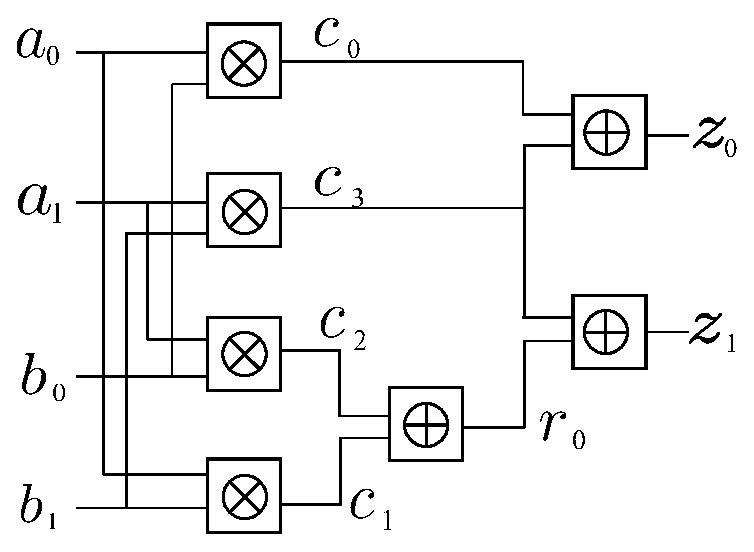
\includegraphics[scale=0.3]{../figures/2bitmultiplier.eps}
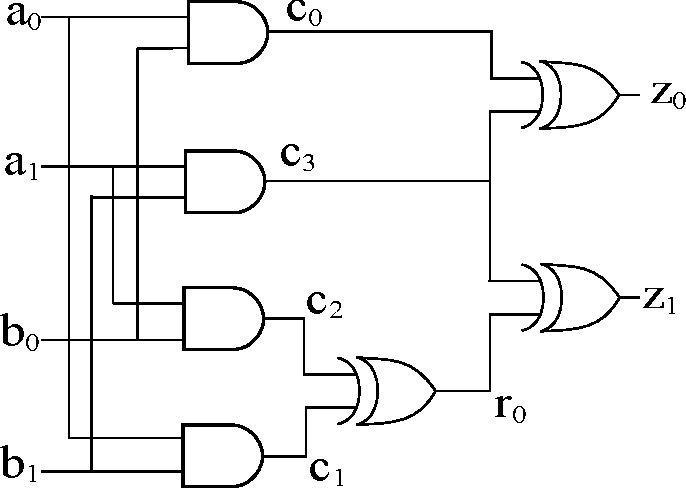
\includegraphics[scale=0.5]{2bitmultiplier_gates.pdf}
}
\caption{\small A 2-bit modulo Multiplier circuit. 
% The gate $\otimes$ is an
%   AND-gate, and $\oplus$ is an XOR-gate; i.e. $\times, +$ modulo 2,
%   respectively.
  } 
\label{fig:mul2bit}
\end{minipage}
\hfill
\begin{minipage}[t]{3.25in}
\vspace{0pt}
%{\small
\begin{align*}
f_1: c_0+a_0 \cdot b_0, \ lm=c_0; ~~~f_2: c_1+a_0 \cdot b_1, \ lm=c_1 \nonumber \\
f_3: c_2+a_1 \cdot b_0, \ lm=c_2; ~~~f_4: c_3+a_1 \cdot b_1, \ lm=c_3 \nonumber \\
f_5: r_0+c_1 + c_2 , \ lm=r_0; ~~~f_6: z_0+c_0 + c_3, \ lm=z_0\nonumber
\end{align*}
\vspace{-0.35in}
\begin{center}
$f_7: z_1+r_0 + c_3, \ lm=z_1$ % \nonumber 
\end{center}
%}
\caption{\small {Polynomials of the circuit under RTTO constitute a GB.
}} 
\label{fig:rel_prime_lt}
\end{minipage}

\end{figure}

%\vspace{-0.1in}
\begin{Example}
\label{ex1}
{\bf Demonstration of the approach:} Consider the circuit given in
Fig. \ref{fig:mul2bit}. 
%Perform a ``reverse topological traversal'' of the circuit. 
Impose RTTO on the circuit. The primary outputs $z_0, z_1$ are both at
level-0, variables $r_0, c_0, c_3$ are at level-1, ~$c_1, c_2$ are at
level-2, and the primary inputs $a_0, a_1, b_0, b_1$ are at
level-3. Order the variables $\{z_0 > z_1\} > \{r_0 > c_0 > c_3\} >
\{c_1 > c_2\} > \{a_0 > a_1 > b_0 > b_1\}$. Using this variable order,
we impose a {\it lex} term order on the monomials. Then all the
polynomials extracted from the circuit have relatively prime leading
terms, as shown in Fig. \ref{fig:rel_prime_lt}, and $G =F = \{f_1, \dots,
f_7\}$ forms a GB. 

Then the GBRs $z_1\xrightarrow{G}_+ a_0\cdot b_0 + a_1\cdot b_1$ and
$z_0\xrightarrow{G}_+a_0\cdot b_1+a_1\cdot b_0 + a_1\cdot b_1$ are
canonical expressions (Boolean polynomials) of the output bits and can
be used for equivalence checking.
\end{Example}


We will now show how to efficiently implement this GBR
$z_i\xrightarrow{G}_+r_i$ on circuits by exploiting the implicit set
representation ZBDDs under the imposition of RTTO. 



\section{Unate Cube Sets \& Boolean Polynomials}
\label{sec:unate}

A Boolean {\it variable} represents a dimension of the Boolean space
$\B^n$, a {\it literal} 
is an instance of a variable $x_i$ or its 
complement $\neg x_i$. A {\it cube} is a product of literals
which denotes a point or a set of points in the Boolean space. A {\it
  cube set} 
consists of a number of cubes, each of which is a combination of
literals. {\it Unate cube sets} allow the use of only positive
literals, not negative/complemented literals. 
%Each cube in a unate
%cube set represents a combination, and each literal represents an
%object selected in the combination.

When cube sets are used to represent Boolean functions, they are
usually {\it binate} cube sets containing negative literals. In binate
cube sets, literals $x_i$ and $\neg x_i$ represent $x_i = 1$ and $x_i = 0$,
respectively; while the absence of a literal implies a {\it don't
  care.} In unate cube sets, literal $x_i$ implies $x_i = 1$ whereas
its absence implies $x_i = 0$. For example, the cube set $\{a,
bc\}$ corresponds to points $(abc): \{111, 110, 101, 100, 011\}$ in
the binate cube set representation, whereas it represents $(abc):
\{100, 011\}$ in the unate cube set representation.

Each monomial of a Boolean polynomial can be viewed as a unate cube --
a product of positive literals -- and a Boolean polynomial as a unate
cube set. Then the GBR $z_i\xrightarrow{G}_+ r_i$ can be interpreted
as %(Boolean) algebra 
operations over unate cube sets, 
%resembling a classical logic synthesis problem, 
as shown below. Let us (re)consider the one-step
division for Boolean polynomials: $f\xrightarrow{g} r$. This division
can be interpreted as:



 \begin{align}
\label{eqns:reduce}
f \xrightarrow{g} r & = f - {{lt(f)} \over {lt(g)}} \cdot g \\
& = ~ f - {{lm(f)} \over {lm(g)}} \cdot g; ~~(\text{coef. 0,1;} ~lt(f)=lm(f))\\ 
& = f + {{lm(f)} \over {lm(g)}} \cdot g; ~~~(-1 = +1 \pmod{ 2})\\
& = f \oplus {{lm(f)} \over {lm(g)}} \cdot g; ~~( as ~+ \pmod{2} =
\oplus) \label{eqns:reduce1}
\end{align}



%% {\small
%% \begin{equation}
%% \label{logic_syn}
%% \begin{split}
%% f \xrightarrow{g} r ~  = & ~ f - {{lt(f)} \over {lt(g)}} \cdot g ~ =  ~ f - {{lm(f)} \over {lm(g)}} \cdot g \\
%% = & ~ f + {{lm(f)} \over {lm(g)}} \cdot g ~ =  ~ f \oplus {{lm(f)} \over {lm(g)}} \wedge g
%% \end{split}
%% \end{equation}
%% }

% $$f \xrightarrow{g} r  = f - {{lt(f)} \over {lt(g)}} \cdot g 
% = ~ f - {{lm(f)} \over {lm(g)}} \cdot g; ~~(\text{coeff. 0,1;}
% ~lt(f)=lm(f))
% $$

% $$= f + {{lm(f)} \over {lm(g)}} \cdot g = f \oplus {{lm(f)} \over
%   {lm(g)}} \wedge g \label{eqns:reduce1}
% $$

%We can replace $lt(f)$ with $lm(f)$ as coefficients are either 0 or
%1. 
Notice that ${{lm(f)} \over {lm(g)}}$ is a unate product of 
literals. i.e. a unate cube. The $\oplus$ operation cancels common
cubes from $f$ and ${{lm(f)} \over {lm(g)}}\cdot g$. The $\cdot$
operation models the modulo 2 product, where the partial products are
added using the $\oplus$  operation. Therefore, we
will implement the reduce operation $f\xrightarrow{g} r$ for Boolean
polynomials as $r = f \oplus {{lm(f)} \over {lm(g)}} \cdot g$ using
an implicit representation particularly suited for such unate cube
operations, i.e. ZBDDs.  

\subsection{Zero Suppressed Binary Decision Diagrams (ZBDDs) for
  Boolean Polynomials}

% A Binary Decision Diagram is a directed graph with two terminal nodes 0 and 1. 
% Each node in the diagram has two edges, solid edge (1-edge) and dotted edge (0-edge). 

Binary decision diagrams (BDDs) \cite{BRYA86} and
their variants 
%such as OKFDDs \cite{drechsler:dac94} and ADDs \cite{add} 
have been used as implicit representations for solving many
Boolean and pseudo-Boolean optimization problems. Zero-suppressed BDDs
\cite{zbdd} are another variant of BDDs that were designed to
efficiently manipulate ``sets of combinations''. A ZBDD is obtained
from an ordered BDD by: i) eliminating those vertices whose 1-edge
(then-edge) is incident on the 0-terminal; and ii) merging isomorphic
subgraphs. Subject to the given variable order, a ZBDD represents a 
Boolean function canonically. \textcolor{red}{Just as with BDDs, every node in a ZBDD
is assigned an index, which corresponds to the variable order imposed
on the diagram.} For a detailed description of ZBDDs and
their capabilities for solving logic optimization and sparse
combinatorial problems, the reader is referred to \cite{zbdd} and
\cite{zbdd_unate}. 

\begin{figure}[hbt]
\centering
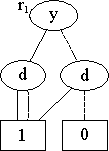
\includegraphics[scale=1]{Preliminaries-Theory/r1_clean.pdf}
\caption{ZBDD for the polynomial $r_1 = yd + y + d$.}
\label{r1}
\end{figure}

In \cite{zbdd_unate}, {\it Minato} demonstrated that ZBDDs are an
efficient data-structure for implicit manipulation (algebra) of unate
cube sets. Fig.~\ref{r1} depicts a ZBDD for the unate cube set
$\{yd,y,d\}$ with the variable order  $y > d$. The paths beginning
from the root node $y$ and terminating in the 1-terminal node
correspond to the cubes of the set. A variable is present in a cube if
its 1-edge lies on the path; otherwise it is absent from the cube
if its 0-edge lies on the path. 
%Since a monomial of a Boolean
%polynomial is a unate cube, we can interpret a Boolean polynomial as a
%set of unate cubes; and each monomial (cube) as a set of
%variables. 
Consequently, the ZBDD of Fig.~\ref{r1} can be construed to
represent the Boolean polynomial $r_1 = yd + y +d$. {\it Minato} has
shown \cite{zbdd}\cite{zbdd_unate} how the set union, intersection and
difference operations can be implemented recursively in the ZBDD
graphs, and they have been implemented using the {\it ite-operator} in
decision diagrams such as the CUDD \cite{cudd} package. We extend
these operations to accommodate the sum and product operations
$\pmod{2}$, i.e. polynomial algebra in $\Ftwo[x_1,\dots,x_n]$, by 
manipulating sets of combinations using ZBDDs. 

%, where each unate cube (monomial) represents one combination,
%and each literal represents an object chosen in the combination.
% -- resembling a
%classical logic synthesis problem. 

%Then the ZBDD can also be used to represent
%polynomials where the monomials can be obtained the same way the cubes
%are obtained for the equivalent set. 

Based on the above discussion, we will: i) model GBR as the
algebra of unate cube sets; ii) use ZBDDs as the implicit
data-structure for this GBR; and iii) devise efficient implementation
of the GBR by exploiting the special structure imposed by RTTO on the
ZBDD graph.  

%For details on the use of unate cube set algebra in classical logic
%synthesis, and its implementation on ZBDDs, we refer the reader to
%\cite{zbdd} \cite{zbdd_unate}. 



\section{Theory}
\label{sec:theory}
We describe the setup for Craig interpolation in the ring
$R=\Fq[x_1,\dots,x_n]$. Partition the variables $\{x_1,\dots,x_n\}$
into disjoint subsets $A, B, C$. We are given two ideals $J_A \subset
\Fq[A,C], J_B \subset \Fq[B,C]$ such that the $C$-variables are common
to the generators of both $J_A, J_B$. {\it From here on, we will
  assume that all ideals include the corresponding vanishing
  polynomials.}  For example, generators of $J_A$ include $\bm{A^q -
A, C^q-C}$ where 
$\bm{A^q-A} = \{x_i^q - x_i: x_i \in A\}$, and so on. Then these
ideals become radicals and we can apply Lemmas \ref{lemma:radical-ff}
and \ref{lemma:project}. We use $\Vac(J_A)$ to denote the variety of
$J_A$ over the $\Fq$-space spanned by $A$ and $C$ variables, 
i.e. $\Vac(J_A) \subset \Fq^A \times \Fq^C$. Similarly,
$\Vbc(J_B)\subset\Fq^B\times\Fq^C$. 

Now let $J = J_A + J_B \subseteq \Fq[A,B,C]$, and suppose that it is
found by application of the Weak Nullstellensatz
(Thm. \ref{thm:weak-ns-ff}) that $\Vabc(J) = \emptyset$. When we
compare the varieties of $J_A$ and $J_B$, then we can consider the
varieties in $\Fq^A\times\Fq^B\times\Fq^C$,  as $\Vabc(J_A) =
\Vac(J_A) \times \Fq^B \subset \Fq^A\times\Fq^B\times\Fq^C$. With this
setup, we define the interpolants as follows.


\begin{Definition}[{\it Interpolants in finite fields}]
\label{def:int}
Given two ideals $J_A \subset \Fq[A,C]$ and $J_B \subset \Fq[B,C]$
where $A,B,C$ denote the three disjoint sets of variables such that 
$\Vabc(J_A) \cap \Vabc(J_B) = \emptyset$. Then there exists an ideal 
$J_I$ satisfying the following properties:
\begin{enumerate}
\item $\Vabc(J_I) \supseteq \Vabc(J_A)$
\item $\Vabc(J_I) \cap \Vabc(J_B) = \emptyset$
\item The generators of $J_I$ contain only the $C$-variables;
 or $J_I \subseteq \Fq[C]$.
\end{enumerate}
We call $\Vabc(J_I)$ the {\bf interpolant} in finite fields of the
pair $(\Vabc(J_A), \Vabc(J_B))$, and the corresponding ideal $J_I$ is
called the {\bf ideal-interpolant}. 
\end{Definition}

As the generators of $J_I$ contain only the $C$-variables, the
interpolant $\Vabc(J_I)$ is of the form $\Vabc(J_I) =
\Fq^A\times\Fq^B\times\Vc(J_I)$. 
%Before we prove the existence of
%$J_I$ and classify the other interpolants, we demonstrate the concept
%of interpolants and ideal-interpolants using an example. 


\begin{Example}
\label{ex:main}
{\it 
Consider the ring $R = \F_2[a, b, c, d,e]$, partition the variables as
% \begin{center}
 $A = \{a\}, B = \{e\}, C = \{b,c,d\}.$
% \end{center}
Let ideals 

\vspace{-0.2in} 

\begin{align*}
 J_A &= \langle ab, bd, bc + c,
 cd, bd + b + d + 1
 \rangle + J_{0,A,C}\\
 J_B &= \langle b,d,ec+e+c+1,
 ec
 \rangle + J_{0,B,C}
 \end{align*}

\vspace{-0.1in} 

where $J_{0,A,C}$ and $J_{0,B,C}$ are the corresponding ideals of vanishing
polynomials. Then, we have

\vspace{-0.2in} 

\begin{align*}
\Vabc(J_A) &= \Fq^B \times \Vac(J_A)  \\
&= (abcde):\{ 01000,00010,01100,10010, \\
& ~~~~~~~~~~~~~~~~~~~~~~ 01001,00011,01101,10011 \} \\
\Vabc(J_B) &= \Fq^A \times \Vbc(J_B) \\
&= (abcde):\{00001,00100,10001,10100\}
\end{align*} 

The ideals $J_A, J_B$ have no common zeros as $\Vabc(J_A) \cap
\Vabc(J_B) = \emptyset$.   
The pair $(J_A, J_B)$ admits a total of 8 interpolants:\\

\begin{minipage}[c]{0.5\textwidth}

{\small
\begin{enumerate}
\item $V(J_S) = (bcd): \{001,100,110\}$\\ 
% is the smallest interpolant,   with ideal-interpolant 
$J_S = \langle cd, b + d+ 1 \rangle$

\item  	 	$V(J_1) = (bcd): \{001,100,110,101\}$\\
$J_1 = \langle cd,bd+b+d+1,bc+cd+c \rangle$ 

\item 
 	$V(J_2) = (bcd): \{001,100,110,011\}$ \\
 	$J_2 = \langle b+d+1 \rangle$ 

\item 
 	$V(J_3) = (bcd): \{001,100,110,111\}$ \\
 	$J_3 = \langle b+cd+d+1 \rangle$ 

\item 
 	$V(J_4) = (bcd): \{001,100,110,011,111\}$ \\
 	$J_4 = \langle bd+b+d+1,bc+b+cd+c+d+1 \rangle$ 

\item 
 	$V(J_5) = (bcd): \{001,100,110,101,111\}$ \\
 	$J_5 = \langle bc+c,bd+b+d+1 \rangle$ 

\item 
 	$V(J_6) = (bcd): \{001,100,110,101,011\}$  \\
 	$J_6 = \langle bd+b+d+1,bc+cd+c \rangle$ 

\item $V(J_L) = (bcd): \{001,011,100,101,110,111\}$ \\
%is the largest  interpolant, with ideal 
$J_L = \langle bd + b + d + 1 \rangle$.

\end{enumerate}
}
\end{minipage}
\hspace{0.3cm}
\begin{minipage}{0.5\textwidth}
% \begin{figure}[hbt]
% \begin{center}
% \centering
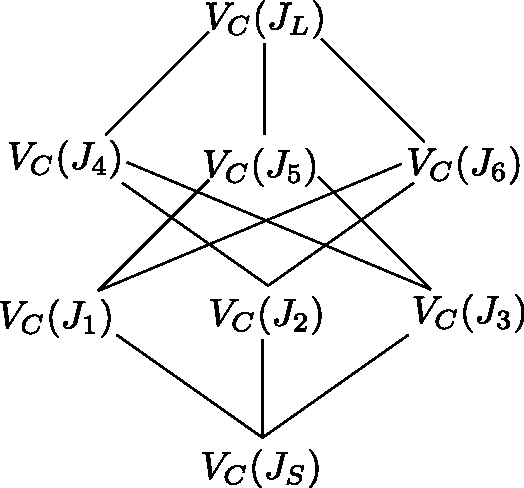
\includegraphics[width=0.8\textwidth]{interpolant_lattice.pdf}
\captionof{figure}{Interpolant lattice}
\label{Fig:int_lat}
% \begin{center}
% \end{figure}
\end{minipage}

It is easy to check  that all $V(J_I)$ satisfy the 3 conditions of
Def. \ref{def:int}. Note also that $V(J_S)$ is the smallest
interpolant, contained in every other interpolant. Likewise, $V(J_L)$
contains all other interpolants and it is the largest. The other
containment relationships are shown in the corresponding interpolant
lattice in Fig. \ref{Fig:int_lat}; i.e. $\Vc(J_1) \subset \Vc(J_5),
\Vc(J_1) \subset \Vc(J_6)$, and so on. 


 %% \begin{align*}
 %% & \Vc(J_1) \subset \Vc(J_5) ~~~~~~~~~~~~ \Vc(J_1) \subset \Vc(J_6) \\
 %% & \Vc(J_2) \subset \Vc(J_4) ~~~~~~~~~~~~ \Vc(J_2) \subset \Vc(J_6) \\
 %% & \Vc(J_3) \subset \Vc(J_4) ~~~~~~~~~~~~ \Vc(J_3) \subset \Vc(J_5)
 %% \end{align*}


}
\end{Example}



%% \begin{Example}
%% \label{example:jajb}
%% Consider the ideal $J_A$ from Example \ref{example:ja} and another
%% $J_B = \langle b,d,ec+e+c+1, ec \rangle$ with the variables of 
%% its generators partitioned as $B = \{e\}$ and $C = \{b,c,d\}$.
%% The intersection of varieties $\Vabc(J_A)$ and $\Vabc(J_B)$ is 
%% empty as,
%% \begin{align*}
%% \Vabc(J_A) &= \Fq^B \times \Vac(J_A)  \\
%% &= (abcde):\{ 01000,00010,01100,10010, \\
%% & ~~~~~~~~~~~~~~~~~~~~~~ 01001,00011,01101,10011 \} \\
%% \Vabc(J_B) &= \Fq^A \times \Vbc(J_B) \\
%% &= (abcde):\{00001,00100,10001,10100\}
%% \end{align*} 

%% Therefore, there must exist an interpolant satisfying the 
%% above three properties. 
%% \end{Example}


\begin{Theorem}
An ideal-interpolant $J_I$, and correspondingly the interpolant $\Vabc(J_I)$, as
given in Def. \ref{def:int}, always exists. 
\end{Theorem}

\begin{proof}
Consider the elimination ideal $J_I = J_A \cap \Fq[C]$. We show $J_I$ satisfies 
the three conditions for the interpolant. 

\par \noindent  \underline{Condition 1}: $\Vabc(J_I) \supseteq
\Vabc(J_A)$. This condition is trivially satisfied due  to
construction of elimination ideals. As $J_I \subseteq J_A$,
$\Vabc(J_I) \supseteq \Vabc(J_A)$.

%% In other words  any point in the $\Vabc(J_A)$ has
%% to satisfy all the polynomials in $J_I$ as $J_I$ is  a subset of
%% polynomials in $J_A$.  

\par \noindent \underline{Condition 2}: $\Vabc(J_I) \cap \Vabc(J_B) =
\emptyset$. This condition  can be equivalently stated as $\Vbc(J_I)
\cap \Vbc(J_B) = \emptyset$ as neither  $J_I$ nor $J_B$ contains any
variables from the set $A$. We prove this condition by
contradiction. Let's assume that there exists a
common point $(\mathbf{b},\mathbf{c})$ in $\Vbc(J_I)$ and $\Vbc(J_B)$.  
We know that the projection of the variety $Pr_A(\Vac(J_A))$ is equal
to the variety of the elimination ideal $\Vc(J_I)$, where $J_I=J_A
\cap \Fq[C]$, due to Lemma \ref{lemma:project}. 
 %% (as $J_A$ is radical). 
Therefore, the point $(\mathbf{c})$ in the variety of $J_I$ can be
extended to a point $(\mathbf{a},\mathbf{c})$ in the variety of
$J_A$. This implies that the ideals $J_A$ and $J_B$ vanish at 
($\mathbf{a},\mathbf{b},\mathbf{c}$). This is a contradiction to our
initial assumption that the intersection of the varieties of $J_A$ and
$J_B$ is empty.  Thus $J_I, J_B$ have no common zeros.

\par \noindent \underline{Condition 3}: The generators of $J_I$
contain only the $C$-variables. This condition is trivially satisfied
as $J_I$ is the elimination ideal obtained by  eliminating
$A$-variables in $J_A$. 
\end{proof}

The above theorem not only proves the existence of an interpolant, but
also gives a procedure to construct one: $J_I = J_A\cap\Fq[C]$. In
other words, compute a reduced Gr\"obner basis $G$ of $J_A$ w.r.t. an
elimination order $A> B > C$ and take $G_I = G \cap \Fq[C]$. Then
$G_I$ gives the generators for the ideal-interpolant $J_I$.

\begin{Example}
{\it 
The elimination ideal $J_I$ computed for $J_A$ from Example \ref{ex:main}
is $J_I = J_S = \langle cd,b+d+1 \rangle$ with variety
$\Vc(J_I)=(bcd):\{001,100,110\}$.  This variety over the variable set
$A$ and $C$ is $\Vac(J_I)=(abcd):\{0001,0100,0110, 1001,1100,1110\}$,
and it contains $\Vac(J_A)$. Moreover, $\Vabc(J_I)$ also has an empty
intersection with $\Vabc(J_B)$. 
}
\end{Example}

%The next theorem proves that this variety $\Vc(J_I)$ is also the
%smallest interpolant, $i.e.$ all other interpolants contain it. 

\begin{Theorem}
\label{thm:smallest}
The interpolant $\Vabc(J_S)$ corresponding to the ideal %-interpolant
$J_S = J_A \cap \Fq[C]$ is the smallest interpolant.
\end{Theorem}

\begin{proof} 
The proof is given in the appendix. 


%% Let $J_I \subseteq \Fq[C]$ be any another ideal-interpolant $\neq
%% J_S$. We show that $\Vc(J_S) \subseteq \Vc(J_I)$. For $\Vc(J_I)$
%% to be an interpolant it must satisfy 
%% \begin{align*}
%% \Vabc(J_A) \subseteq \Vabc(J_I)
%% \end{align*}
%% which is equivalent to 
%% \begin{align*}
%% I(\Vabc(J_A)) &\supseteq I(\Vabc(J_I)) \\
%% \implies J_A &\supseteq J_I  
%% \end{align*}
%% due to Theorem \ref{thm:strong-ns}.
%% %% as $J_I$ is radical so $I(\Vabc(J_I)) = J_I)$. 
%% As the generators of $J_I$ only contain polynomials in $C$-variables,
%% this relation also holds for the following
%% \begin{align*}
%% J_A \cap \Fq[C] &\supseteq J_I \\
%% \implies J_S &\supseteq J_I \\
%% \implies \Vc(J_S) &\subseteq \Vc(J_I).
%% \end{align*} 
\end{proof}

%After proving that the elimination ideal $J_A \cap \Fq[C]$ is the
%smallest interpolant, 
Now we discuss how the largest interpolant can be
computed. For this, we will make use of quotients of ideals. 

\begin{Definition}
\label{def:quo}
({Quotient of Ideals}) If $J_1$ and $J_2$ are ideals in a ring $R$,
then $J_1:J_2$ is the set 
%  \begin{equation}
  $\{f \in R \ |\ f\cdot g \in J_1, \forall g \in J_2\}$ %\nonumber
%  \end{equation}
and is called the {\bf ideal quotient} of $J_1$ by $J_2$.
\end{Definition}

We use ideal quotients to compute the complement of a variety. Given
an ideal $J' \subset R$ containing the vanishing polynomials, suppose
we need to find an ideal $J$ such that $V(J) = \Fq^n - V(J') = V(J_0)
- V(J')$, where ``$-$'' corresponds to the set difference
operation. Then $J = J_0 : J'$ (see Theorem III.2 and Corollary III.1
in \cite{xiaojun:hldvt2016} for a proof outline). Once again, the
Gr\"obner basis algorithm can be used to compute $J_0:J'$ 
\cite{ideals:book}.  

\begin{Theorem}
\label{thm:large}
Consider the elimination ideal $J'_L = J_B \cap \Fq[C]$. The
complement of the variety $\Vc(J'_L)$,  computed as $\Fq^C - \Vc(J'_L)$,
is the largest interpolant.
\end{Theorem}

\begin{proof} Proof is given in the appendix. 

%% We first prove that the interpolant computed by
%% complementing $\Vc(J'_L)$  as $\Fq^C - \Vc(J'_L)$ is indeed a valid
%% interpolant. As $J'_L$ is the elimination ideal computed from $J_B$,
%% $\Vbc(J'_L) \supseteq \Vbc(J_B)$. This in turn implies that the
%% complement of $V(J'_L)$ cannot intersect with $V(J_B)$ at any
%% point. This proves condition 2 for $\Fq^C - \Vc(J'_L)$ to be a
%% valid interpolant.  

%% For condition 1, we need to prove that
%% \begin{align*}
%% \Vac(J_A) \subseteq \Fq^A \times (\Fq^C - \Vc(J'_L))
%% \end{align*}
%% This can be restated as
%% \begin{align*}
%% \Vac(J_A) \cap \Fq^A \times \Vc(J'_L) = \emptyset
%% \end{align*}
%% Let us assume (by contradiction) that there exists a common point 
%% $(\mathbf{a},\mathbf{c})$ in $\Vac(J_A)$ and $\Fq^A \times
%% V_C(J'_L)$. As the projection $Pr_B(\Vbc(J_B))$ on the
%% $C$-variables is equal to  the variety of the elimination ideal
%% $\Vc(J'_L)$, a point $(\mathbf{c}) \in \Vc(J'_L)$ can be  extended to
%% some point $(\mathbf{b},\mathbf{c})$ in $\Vbc(J_B)$. This implies that
%% the point $(\mathbf{a},\mathbf{b},\mathbf{c})$ is a common point in
%% $\Vabc(J_A)$ and $\Vabc(J_B)$, which is a contradiction to our initial
%% assumption. Therefore condition 1 of Def. \ref{def:int} is satisfied
%% too and $\Fq^C - \Vc(J'_L)$ is indeed an interpolant. 

%% \par \noindent Next we prove that $\Fq^C - \Vc(J'_L)$ is the largest
%% interpolant. Consider an arbitrary ideal-interpolant $J_I$. We want to
%% prove $\Vc(J_I) \subseteq \Fq^C - \Vc(J'_L)$, or equivalently to prove
%% $\Vc(J_I) \cap \Vc(J'_L) = \emptyset$. Let us assume (by contradiction) 
%% that there exists a common point $(\mathbf{c})$ in $\Vc(J_I)$ and
%% $\Vc(J'_L)$. As $J'_L$ is the elimination ideal of $J_B$, this point
%% can be extended to some point $(\mathbf{b},\mathbf{c})$  
%% in $\Vbc(J_B)$. This in turn implies that $(\mathbf{b},\mathbf{c})$ is
%% a common point in  $\Vbc(J_B)$ and $\Fq^B \times \Vc(J_I)$. This is a
%% contradiction as an interpolant cannot intersect with the variety of
%% $J_B$. Hence, $\Fq^C - \Vc(J'_L)$ is the largest interpolant and it
%% contains all other interpolants.

\end{proof}

Let $J_L$ be the radical ideal corresponding to the largest
interpolant $\Vc(J_L) = \Fq^C - \Vc(J'_L)$. This ideal-interpolant
$J_L$ can be computed as $J_L = (J_{0,C}:J'_L)$, where $J_{0,C}$ is
ideal of vanishing polynomials in $C$-variables.  


\begin{Example}
{\it 
The ideal-interpolant $J_L = \langle bd + b + d + 1 \rangle$ in 
Example~\ref{ex:main} is computed as:
\begin{itemize}
	\item First compute the ideal $J'_L = J_B \cap \Fq[C]$ which results in 
	$J'_L = \langle b,d \rangle$.
	\item Then compute $J_L$ as $J_L = J_{0,C}: J'_L$ which results in
	$J_L = \langle bd + b + d + 1 \rangle$
\end{itemize}
The variety $V_C(J_L)=(bcd):\{001,011,100,101,110,111\}$ and it is the
largest interpolant for the given pair ($J_A,J_B$). 
}
\end{Example}

\begin{Lemma}
\label{noofinter}
The total number of interpolants for the pair ($J_A,J_B$) is
$2^{|SM(J_D)|}$, where $J_D = (J_L:J_S)$. 
\end{Lemma}

\begin{proof}
The proof is given in the appendix. 

%% The smallest and the largest interpolants are $\Vc(J_S)$ and $\Vc(J_L)$,
%% respectively. The set difference $\Vc(J_L) - \Vc(J_S)$ is also a
%% variety of some ideal $J_D$, which can be computed as
%% $J_D=(J_L:J_S)$. By selecting different subsets of $\Vc(J_D)$ and
%% adding them to $\Vc(J_S)$, we can generate all the 
%% interpolants. Consider, 
%% \begin{align*}
%% \label{eqn:pwsetjd}
%% \binom{|\Vc(J_D)|}{0} + \binom{|\Vc(J_D)|}{1} + \cdots + \binom{|\Vc(J_D)|}{|\Vc(J_D)|} = 2^{|\Vc(J_D)|}
%% \end{align*}
%% where the term $\binom{|\Vc(J_D)|}{0}$ denotes that no point is selected from $\Vc(J_D)$ and results in 
%% $\Vc(J_S)$ as the ideal-interpolant. On the other hand, the term $\binom{|\Vc(J_D)|}{|\Vc(J_D)|}$ is equivalent 
%% to selecting  all the points from $\Vc(J_D)$ and results in $J_L$ as 
%% the ideal-interpolant. So the number of interpolants is equal to
%% $2^{|\Vc(J_D)|}$. Theorem \ref{thm:count} further tells us that the 
%% cardinality of a variety of an ideal is equal to the number of
%% standard monomials of that ideal, therefore, number of interpolants $=
%% 2^{|SM(J_D)|}$.  

\end{proof}

\begin{Example}
\label{ex:jd}
{\it 
From Example~\ref{ex:main}
$J_L = \langle bd + b + d + 1 \rangle$ and $J_S = \langle cd, b + d+
1\rangle$. 
Computing $J_D = J_L : J_S$ gives $J_D = \langle
d+1,bc+b+c+1,c^2+c,b^2+b \rangle$, where the variety $\Vc(J_D)=\Vc(J_L)-\Vc(J_S)
=(bcd):\{011,101,111\}$. 

The standard monomials for $J_D$ are $SM(J_D) = \{1,b,c\}$. Therefore,
the total number of interpolants for the given pair ($J_A,J_B$) is
$2^{|\{1,b,c\}|}=2^3=8$. 
}
\end{Example}


\subsubsection{The structure of the interpolant lattice:} Note that
our results do provide some insights into the structure of the
interpolant lattice. Let $l = |SM(J_D)|$. Then, the height of the
interpolant lattice is $l + 1$, and the number of elements (interpolants) at each
level $i$ is $l \choose i$, $0\leq i \leq l$. Notice also that the size (height and
width) of the interpolant lattice is independent of the number of
variables in the set $C$, and depends only on $|SM(J_D)|$. 

%% Next we describe a procedure for enumerating all of these interpolants using the $SM(J_D)$.
%% Let's say there are $l$ standard monomials, $\{m_1,\dots,m_l\}$ in the set $SM(J_D)$. Consider
%% a polynomial $f_i$ constructed using the linear combination of $\{m_1,\dots,m_l\}$ as,
%% \begin{center}
%% $f_i = \lambda_1\cdot m_1 + \lambda_2\cdot m_2 +\cdots+ \lambda_l\cdot m_l$
%% \end{center} 
%% where each $\lambda_i \in \mathbb{F}_2$ $i.e.$ $\lambda_i \in \{0,1\}$.
%% There can be exactly $2^l$ unique polynomials obtained in this way.
%% We can then obtain all the ideal-interpolants $I_j$ as,
%% \begin{center}
%% $I_j = J_S\cdot(J_D + \langle f_i \rangle)$
%% \end{center}
%% where $\langle f_i \rangle$ is the ideal generated by the polynomial $f_i$.

%\documentclass{article}
%\documentclass[10pt,twocolumn]{IEEEtran}
%\usepackage[a4paper, margin=1in]{geometry}%lmargin=1in, rmargin=1in, tmargin=1in, bmargin=1in]{geometry}
%\usepackage{algorithm}
%\usepackage{algpseudocode}
%\usepackage{svg}
%\usepackage{xcolor}
%\usepackage{multirow}
%\usepackage{booktabs}
%\bibliographystyle{plain}
%\usepackage{float}
%\usepackage{boldline}
%\usepackage{pbox}
%\usepackage{tabularx}
%\usepackage{graphicx}
%\usepackage{amsmath}
%\usepackage{amsfonts}

%\begin{document}

\section{Experimental Results}
\label{sec:exp}
\iffalse
%\iffalse
This section presents the results of reducing modulo multiplier
circuits used in cryptography using our implementation. The
experiments are performed on a 3.5GHz Intel 
Core\textsuperscript{TM} i7-4770K Quad-Core CPU with 32 GB of RAM. There are
two architectures that implement these multipliers, namely Mastrovito
and Montgomery. 
Mastrovito multipliers compute $Z = A\times B \pmod{
  P}$
%take $\{A,B\} =
%\{a_0,a_1,\dots,a_{k-1},b_0,b_1,\dots,b_{k-1}\}$ as $k$-bit inputs and
%produce $Z = \{z_0,z_1,\dots,z_{k-1}\}$ as $k$-bit output. The multiplier
%performs $Z = A \times B \pmod{P}$, 
where $P$ is a given primitive polynomial for the datapath size
$k$. 
%The procedure 
%involves computing the product $S=A\times B$ using an array multiplier
%and then reducing it $\pmod{P}$ to obtain $Z$. We perform experiments
%on \textit{flattened} netlists of these circuits.  
Montgomery multipliers perform fast modular multiplication without
explicitly performing the reduction $\pmod{P}$. 
%They are more
%efficient than the Mastrovito multipliers when several modulo
%multiplications are required as in the case of exponentiation in
%cryptosystems. 
Fig.~\ref{montfig} shows the structure of a Montgomery
multiplier. Each MR block computes $A\cdot B\cdot R^{-1}$, where $R$
is selected as a power of a base ($\alpha^{k}$). We denote the leftmost
two blocks as Block A (upper) and B (lower), the middle block as Block
C and the output block as Block D. We have presented results for GBR
on both \textit{flattened} and \textit{hierarchical} netlists of these
multipliers. 

\begin{figure}[H]
  \centering
  %\def\svgwidth{340pt}
  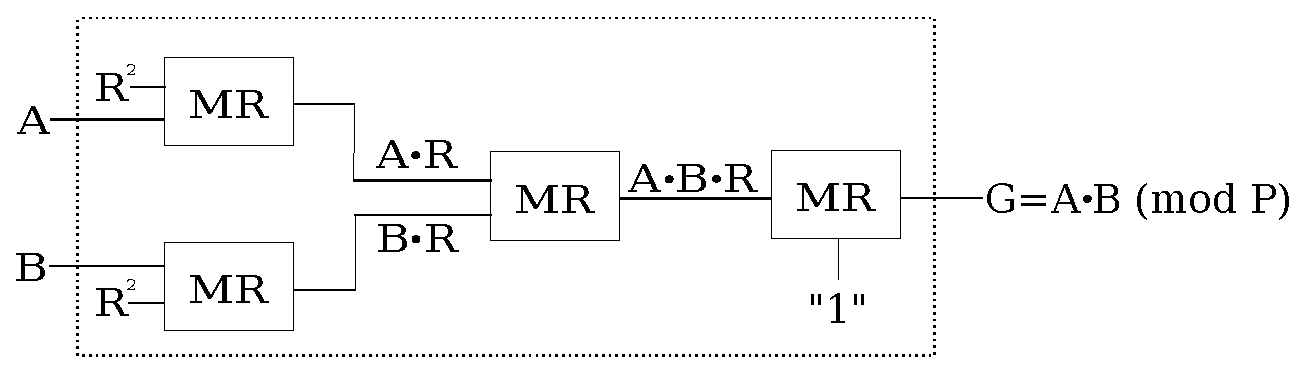
\includegraphics[scale=0.34]{new_mmcircuit}
  \caption{Montgomery multiplication}
  \label{montfig}
  \end{figure}

 
Table~\ref{masmm} provides the statistics on the time, ZBDD size, and
savings in the number of monomial cancellations achieved by our
approach as compared to classical symbolic algebra methods, for
Mastrovito multiplier circuits. The time reported is the total time
required to perform the reduction, $z_i \xrightarrow{G}_+ r_i$, for
all $i = 0,\dots,k-1$. The columns 
\textit{F4}, \textit{PB}, and \textit{ZR} represent the time taken in
seconds by F4 style reduction, PolyBori (version 0.8.3) and our
implementation respectively. \textit{MN} represents the maximum size
of any ZBDD encountered during reduction of any output-bit, while
\textit{MR} represents the maximum size of the ZBDD among all final
remainders $r_i$. \textit{CS} represents the
number of iterations saved during reduction due to our implicit
method. PolyBori throws a segmentation fault for the multiplier with
$k = 571$ which is depicted as \textit{CR} in the table. Our approach
is orders of magnitude faster than both \textit{F4} and \textit{PB}. 

Table~\ref{montmm} provides the same statistics for \textit{flattened}
Montgomery multipliers. The data for \textit{MN} and \textit{CS}
columns in  case of  $k=571$ could not be procured as both these
operations require traversal along ZBDDs (using the procedure {\tt
  Cudd\_zddDagSize()} and {\tt Cudd\_zddNextPath}). As there is a huge
number of large-sized intermediate ZBDDs produced during this
reduction, traversing along each path of every ZBDD is
infeasible. Also, the reduction times for $k=283$ is inordinate when
compared to other datapath sizes, which is purely due to  the
structure of the circuit.  


%The reduction times for $k=283$ is inrodindate when compared to other datapath sizes, which is purely due to the structure of this circuit.

%Table~\ref{montblockmm} and~\ref{montblockstats} depicts the comparison of time, ZBDD size, and monomial savings across \textit{Montgomery} Flat multiplier circuits with different field sizes. \textit{F4}(F4 style abstraction)*reference to Tim's paper*, \textit{PB}(PolyBori), and \textit{ZR}(ZBDD Reductions) represents the time in seconds for the respective implementations. \textit{MN}(Max Nodes) represents the maximum number of ZBDD size encountered, while \textit{MR}(Max Remainder) represent the maximum size for any remainder after the reductions. \textit{CS}(Cancellation Savings) signifies the total amount of monomial savings with our implementation.

%Table~\ref{montblockmm} depicts the comparison of ZBDD max size, remainders, and monomial savings across \textit{Montgomery} Block multiplier circuits with different block sizes, given different field sizes. For a given Block and field size, \textit{MN}(Max Nodes) represents the maximum number of ZBDD size encountered, while \textit{MR}(Max Remainder) represents the maximum size for any remainder while doing reductions with our implementation. \textit{CS}(cancellation savings) signifies the total amount of monomial savings with our implementation.

Table \ref{montblockmm} present the
statistics for hierarchical Montgomery multipliers for the blocks A,
B, C, and D. The experiment first reduces the outputs of a block
modulo the gates of that block, and then reduces the primary outputs
modulo these four sets of remainders (ZBDDs), thus exploiting the
hierarchy of these circuits. Table~\ref{montblockmm} shows the time
for reduction of each block and the time for reducing the primary
outputs across the four levels. The  time for reducing the primary
outputs across  levels in case of F4 implementation is $<$1 second,
and is not explicitly mentioned in the table. The row labeled
\textit{Total} presents the sum of time of reduction across levels and
the maximum reduction time for each block (as the reductions for the
four levels are independent of each other and are done in
parallel). The datapath sizes of these circuits correspond to
NIST-specification in cryptography with $k = 163,\dots,571$ bits.

%\par The reduction time presented in this section is obtained by reducing each output bit sequentially. These runtimes can be further improved by running these reductions in parallel.

%% The reduction times for small integer arithmetic array multipliers are
%% presented in Table \ref{intmm}. There is an 8x increase in time when
%% moving from $n-1$ datapath size to $n$-bits, which is an exponential
%% increase. Performing detailed analysis of a 7x7 multiplier reveals
%% that, when reducing the $z_{13}$ bit (MSB) and $z_{12}$ bit of this
%% circuit, the maximum number of monomials encountered are 429,889 and
%% 897,955. Of these, 269,120 monomials are {\it common to both output
%%   bits}. This implies that integer multipliers require a word-level
%% decision procedure, as given in \cite{ciesielski:dac2015}
%% \cite{rolf:date16}, that account for the cancellation of these
%% monomials across multiple bits in one word-level expression. Our
%% results show that bit-level techniques cannot efficiently verify
%% integer arithmetic circuits, but are very efficient for finite-field
%% arithmetic circuits.    
%\fi


%\iffalse
%%%%%%%%%%%%%%%% Mas Multipliers %%%%%%%%%%%%%%%%%%%
\iffalse
\begin{table}[H]
\centering
%\caption{Mastrovito Multipliers (Time in seconds, \# of nodes, \# of redundant monomials in $k$)  (K = $10^3$, M = $10^6$)}
\caption{Mastrovito Multipliers (Time in seconds)  TO = 3 days, (P):Parallelization, (WP):Without Parallelization}
\label{masmm}
\begin{tabular}{| c | c | c | c | c | c | c |} \hline
%\multirow{2}{*}{\textbf{Input}} & \multirow{2}{*}{\textbf{Abstraction}} & \multicolumn{3}{ c |}{\textbf{ZBDD reduction(ZR)}}  &  \multirow{2}{*}{\textbf{ZR improved}}\\ \cline{3-5}
% & &Building ZBDDs&Reduction&Total&\\ \hline
\textbf{Datapath(k)}&\textbf{\# of Gates} & \textbf{F4} &\textbf{\#T}&\textbf{CX(P)} & \textbf{PB(WP)} & \textbf{ZR(WP)}\\ \hline
163 &153K& 1,443 &30& 110 &70& 9  \\ \hline 
233 &167K& 1,913 &30&169 &105& 9 \\ \hline
283 &399K& 11,116 &30&496&316& 37 \\ \hline
409 &508K& 17,848 &30& 909& 596&39 \\ \hline
571 &1.6M& 192,032 &10&4,245& CR&566 \\ \hline 


\end{tabular}
\end{table}
\fi

%%%%%%%%%%%%%%%%%%%%%%%%%%%%%%%%%%%%%%%%%
%%%%%%%%%%%%%%%% Mont Multipliers %%%%%%%%%%%%%%%%%%
\iffalse
\begin{table}[H]
\centering
%\caption{Montgomery Flat Multipliers (Time in seconds) (K = $10^3$, M = $10^6$, B = $10^9$, No. of threads = T)}
\caption{Montgomery Multipliers (Time in seconds)  TO = 3 days, (P):Parallelization, (WP):Without Parallelization}
\label{montmm}
\begin{tabular}{| c | c | c | c | c | c | c |} \hline
%\multirow{2}{*}{\textbf{Input Bit-width}} & \multirow{2}{*}{\textbf{Abstraction}} & \multicolumn{3}{ c |}{\textbf{ZBDD reduction(ZR)}}  &  \multirow{2}{*}{\textbf{ZR improved}} \\ \cline{3-5}
% & &Building ZBDDs&Reduction&Total& \\ \hline
\textbf{Datapath(k)}&\textbf{\# of Gates} & \textbf{F4} & \textbf{\#T} &\textbf{CX(P)}& \textbf{PB(P)}  &\textbf{ZR(P)} \\ \hline
163 & 184K&6,897 & 20&1,142&5,590&6,224 \\ \hline 
233 & 329K&63,805 &10 &316& 578&468\\ \hline
283 & 488K&TO &10&15,055  &108,168& 129,904 \\ \hline
409 & 1.0M&TO & 3&2,609 &9,350&8,959\\ \hline
571 & 1.97M&TO & 3 &estimated 4days (TO) &CR&43,813 \\ \hline 

\end{tabular}
\end{table}
\fi
%%%%%%%%%%%%%%%%%%%%%%%%%%%%%%%%%%%%%%%%%
\fi

This section presents the results of using our implementation
(Algorithm~\ref{multimon}) for formal verification and equivalence
checking of circuits used in cryptography. We compare our results
against: i) F4-style reduction~\cite{pruss:tcad} which models the
reduction as Gaussian elimination on a coefficient matrix;   ii)
Parallelized approach for performing reductions on Galois field 
multipliers~\cite{cunxi:aspdac17};  and iii) PolyBori's \cite{polybori:2009}
%% that uses the conventional
reduction procedure with ZBDDs as
underlying data structure. For all tools and experiments, RTTO $>$ is
used for constraint representation. 
 The experiments are performed on a 3.5GHz
Intel Core\textsuperscript{TM} i7-4770K Quad-Core CPU with 32 GB of
RAM. Experiments are conducted for verification of finite field
multipliers and polynomial computation modules used as cryptography
primitives. The data-path sizes {$k$} are selected according to
cryptography standards recommended by U.S. National Institute of
Standards and Technology (NIST). 
% Modular multiplication is an important computation used in cryptography. 
% We have performed experiments with two architectures for this multiplication, namely Mastrovito and Montgomery. 

\subsection{Mastrovito Multipliers}

Modular multiplication is an important computation used in
cryptography. A Mastrovito multiplier architecture can be employed for
performing this computation over the finite field of $2^k$ elements,
i.e. $\mathbb{F}_{2^k}$. Mastrovito multipliers compute $Z = A\times B \pmod{
  P(x)}$ where $P(x)$ is a given primitive polynomial for the datapath size
$k$. The product $A \times B$ is computed using an array multiplier
architecture, and then the result is reduced modulo $P(x)$. The
following example demonstrates the Mastrovito multiplier
computation~\cite{lv:tcad2013}. 
%take $\{A,B\} =
%\{a_0,a_1,\dots,a_{k-1},b_0,b_1,\dots,b_{k-1}\}$ as $k$-bit inputs and
%produce $Z = \{z_0,z_1,\dots,z_{k-1}\}$ as $k$-bit output. The multiplier
%performs $Z = A \times B \pmod{P}$, 

%The procedure 
%involves computing the product $S=A\times B$ using an array multiplier
%and then reducing it $\pmod{P}$ to obtain $Z$. We perform experiments
%on \textit{flattened} netlists of these circuits.  

\begin{Example}
\label{exp1}
{\it 
Consider the finite field $\mathbb{F}_{2^4}$ where the operand size is 4. Let the inputs be:
$A=a_0+a_1\cdot \alpha+a_2\cdot \alpha^2+a_3\cdot \alpha^3$ and
$B=b_0+b_1\cdot \alpha+b_2\cdot \alpha^2+b_3\cdot \alpha^3$, and 
 the primitive polynomial be $P(x)=x^4+x^3+1$ with $\alpha$ as its
 root so that $P(\alpha) = 0$.  
 % We have to perform the multiplication $Z =A\times B \pmod{ P(x) }$. 
The constituent bits of $A$  and $B$ are $\{a_0, \dots, a_3\}$ and
$\{b_0, \dots, b_3\}$ respectively, which are the primary inputs of
the circuit. First, we perform the multiplication $A\cdot B$ as:

%\vspace{-0.2in}

\vspace{0.05in}

{\small
{\begin{tabular}{c c c c c c c c}
%\vspace{-0.2in}
  &   &   & $a_3$ & $a_2$ & $a_1$ & $a_0$  \\ 
 $\times$&   &   & $b_3$ & $b_2$ & $b_1$ & $b_0$  \\ 
 \hline
 &   &   & $a_3\cdot b_0$ & $a_2 \cdot b_0$ & $a_1\cdot b_0$ & $a_0\cdot b_0$ \\
 &  & $a_3\cdot b_1$ & $a_2\cdot b_1$ & $a_1 \cdot b_1$ & $a_0\cdot b_1$ &   \\
 & $a_3\cdot b_2$ & $a_2\cdot b_2$ & $a_1\cdot b_2$ & $a_0\cdot b_2$ &  &   \\
 $a_3\cdot b_3$ & $a_2\cdot b_3$ & $a_1\cdot b_3$ & $a_0\cdot b_3$ &  &  &   \\
 \hline
 $s_6$& $s_5$  & $s_4$  & $s_3$ & $s_2$  & $s_1$   & $s_0$ 
% \vspace{-0.2in}
\end{tabular}}
}

\vspace{0.05in}

The result $S = s_0+s_1\cdot \alpha + s_2\cdot \alpha^2 + s_3\cdot
\alpha^3 + s_4\cdot \alpha^4 + s_5\cdot \alpha^5 + s_6\cdot \alpha^6$,
where, $s_0  =  a_0\cdot b_0, ~~s_1  =  a_0\cdot b_1 + a_1\cdot b_0,
~~s_2 = a_0\cdot b_2 + a_1\cdot b_1 + a_2\cdot b_0$, and so on. Here
the multiply ``$\cdot$'' and add ``$+$'' operations are performed
modulo 2, and hence implemented in a circuit using AND and XOR
gates. As the coefficients are always reduced $\pmod 2$ in $\mathbb{F}_{2^k}$, there are no carry-chains
in the design. Next, the result $S$ is reduced modulo the primitive
polynomial $P(x) = x^4 + x^3 + 1$, as:
% where the final output of the circuit is denoted by $G(x)  = g_3x^3
% + g_2x^2 +g_1x + g_0$.  

\vspace{0.05in}

{\small
{\begin{tabular}{|c c c c | l }
  $s_3$   &$s_2$    &$s_1$   &$s_0$   &   \\
 \hline
 $s_4$    &$0$    &$0$   &$s_4$   &$s_4\cdot \alpha^4 \pmod{P(\alpha)} = s_4 \cdot (\alpha^3 + 1)$\\
 $s_5$    &$0$    &$s_5$   &$s_5$     &$s_5\cdot \alpha^5 \pmod{P(\alpha)} = s_5\cdot (\alpha^3+ \alpha + 1)$\\
 $s_6$    &$s_6$    &$s_6$   &$s_6$     &$s_6\cdot \alpha^6 \pmod{ P(\alpha)} = s_6\cdot( \alpha^3 + \alpha^2 + \alpha + 1)$\\
 \hline
 $z_3$    &$z_2$    &$z_1$   &$z_0$   &
 \end{tabular}\par}
}

\vspace{0.05in}

The primary output of the circuit is: $Z = \{z_0, \dots, z_3\}$,
represented as $Z =  z_0 + z_1 \alpha + z_2
\alpha^2 + z_3 \alpha^3$; where  $z_0=s_0+s_4+s_5+s_6; ~~z_1=s_1+s_5+s_6;
~~z_2=s_2+s_6; ~~z_3=s_3+s_4+s_5+s_6$. 
}
\end{Example}

\par Table~\ref{masmmsyn} provides the results for the reductions $z_i
\xrightarrow{G}_+ r_i$ for Mastrovito multipliers for each output bit
$z_i, \textcolor{red}{0\leq i \leq k-1}$. The benchmarks are taken
from~\cite{lv:tcad2013} and optimized using ABC~\cite{ABCtool} with
the commands $resyn2$ and $dch$ as mentioned
in~\cite{cunxi:aspdac17}. Algorithm~\ref{multimon} reduces each output
bit independently of other bits. Therefore, we have presented the
results obtained by running our reduction algorithm both parallelly and
sequentially for each output bit. Similarly, the results for
implementation in PolyBori are also presented for both cases. The
implementation presented in \cite{cunxi:aspdac17} is already
parallelized. We parallelized the PolyBori and our implementation by
creating individual processes for  each output bit $z_i$ that has its
own set of variables and gate polynomials, $poly\_list$
(Algorithm~\ref{multimon}). The maximum number of parallel processes
is decided upon the memory usage of each process ($i.e.$ reducing one
bit) for our implementation and the total available memory. The larger
benchmarks are run with fewer parallel processes as they consume more
memory. 
% As ZBDDs are more complex data structures compared to those used in~\cite{cunxi:aspdac17}, the upper limit of memory usage for each bit is set by our implementation. For instance, an individual process in the reduction of 283-bit multiplier can take upto $\sim 3\%$ of available memory as compared to $\sim 6\%$ in the case of 409-bit mulitplier. Therefore, we run the all the implementations with 20 parallel processes for 283-bit multiplier but only with 10 for 409-bit multiplier. 
\par In the table, the column \#T represents the number of parallel
processes. (S) and (P) refer to the cases when the experiments are run
sequentially and parallelly for the output bits $z_i$, respectively.  

%%%%%%%%%%%%% Syn Mas Multipliers %%%%%%%%%%%%%%%%%%%
%\iffalse
\begin{table}[H]
\centering
%\caption{Synthesized Mastrovito Multipliers (Time in seconds, \# of nodes, \# of redundant monomials in $k$)  (K = $10^3$, M = $10^6$)}
\caption{Mastrovito Multipliers (Time in seconds);  $k$ = Datapath Size, \#Gates = No. of gates, \#T = No. of threads, Time-Out = 30 hrs, (P): Parallel Execution, (S): Sequential Execution, K = $10^3$, M = $10^6$, PB: PolyBori, ZR: Algorithm~\ref{multimon}}
\label{masmmsyn}
\begin{tabular}{| c | c || c | c | c | c | c | c | c |} \hline
%\multirow{2}{*}{\textbf{Input}} & \multirow{2}{*}{\textbf{Abstraction}} & \multicolumn{3}{ c |}{\textbf{ZBDD reduction(ZR)}}  &  \multirow{2}{*}{\textbf{ZR improved}}\\ \cline{3-5}
% & &Building ZBDDs&Reduction&Total&\\ \hline
\multirow{2}{*}{$\boldsymbol{k}$}&\multirow{2}{*}{\textbf{\#Gates}}&\multirow{2}{*}{\textbf{F4~\cite{pruss:tcad}}}& \multirow{2}{*}{\textbf{\#T}}&\multirow{2}{*}{\textbf{~\cite{cunxi:aspdac17}(P)}}& \multicolumn{2}{ c |}{\textbf{PB}}&\multicolumn{2}{ c |}{\textbf{ZR}}\\ \cline{6-9}
&&&&&\textbf{(P)}&\textbf{(S)}&\textbf{(P)}&\textbf{(S)} \\ \hline
64 &11.5K&1.3&20& 3.70&3.60& 2.21&0.73 &\textbf{0.27}\\ \hline 
% 96 &25.6K&&20& 11.66&10.25&6.92 &2.04 &\textbf{0.66}\\ \hline 
128 &46K&9.89&20&27.54 &23.99&16.76& 5.08 &\textbf{1.63}\\ \hline 
163 &73.5K&32.61&20& 55.96&48.67&33.72&  11.41&\textbf{3.11}\\ \hline 
233 &122K&86.30& 20&127.61&112.96 &77.23& 21.77&\textbf{3.63}\\ \hline
283 &193K&274.68& 20&253.05&227.77&157.45& 49.89&\textbf{11.41}\\ \hline
409 &386K&2,528.5& 10&716.80 &659.64&426.92& 163.52&\textbf{17.68}\\ \hline
571* &1.6M & TO &3 & 5,331&CR&CR&2,126.7& \textbf{566.4}\\ \hline
\end{tabular}
\end{table}
%\fi{}

%%%%%%%%%%%%%%%%%%%%%%%%%%%%%%%%%%%%%%%%%
\par The 571-bit multiplier could not be synthesized and mapped with
the given memory due to its large size. Therefore, we have provided
results for a structured (but unoptimized) 571-bit multiplier
benchmark. Our implementation outperforms the explicit approaches
of~\cite{pruss:tcad} and~\cite{cunxi:aspdac17} for Mastrovito
multipliers and also PolyBori. For the 571-bit multiplier, the
implementation of~\cite{pruss:tcad} does not finish for the given time
period of 30 hours and the PolyBori implementation crashes (CR).
\textcolor{red}{The maximum memory consumption for Mastrovito multipliers
when GBR is performed sequentially varies from 131.6 MB for 64-bit
operands to 8.1 GB for 571-bit operands.} 

\par An interesting point to note in Table~\ref{masmmsyn} is that
our implementation takes less time when we are running it
sequentially. There is a certain overhead involved when we declare
variables and build ZBDDs for each gate of the circuit. In the case of
Mastrovito multipliers benchmarks, this overhead is substantially
greater than the reduction time for each output bit. Therefore, when
we run these benchmarks parallely this overhead increases the overall
run time.  
% For example, for the 64-bit multiplier the overhead is 22.09 ms (when running it sequentially), whereas the reduction time for most of the bits is $\sim 0.30$ ms. The sequential reduction time with these values is $22.09 + 64 (0.3) = 41.29$ ms. On the other hand, with 20 processes this time is approximately $(64/20)(22.09 + 0.3) = 71.65$ ms. 
% There are other factors involved too, $e.g.$ CUDD package maintains an internal cache that helps avoid duplicate computations. When performing reduction sequentially the operations involving fanouts can be stored in the cache and used during the reduction of different output bits. 
 
{\bf Efficiency of our approach:} The efficiency of our approach is
attributed to the implicit data-structure and the number of iterations
($while$ loop in Algorithm~\ref{singlemon}) that are saved while
performing the GBR. Table~\ref{monomsave} shows  
the number of explicit monomial cancellations
that are {\it avoided in our approach} by exploiting the structure of the
ZBDDs, when applied for the GBR $z_i\xrightarrow{G}_+ r_i$ for
verification of Mastrovito multipliers.  
%The  number of monomials
%that are generated and eventually gets canceled ($2\cdot(yd + y)$
%expression in Eqn.~\ref{mteq})  due to operations being performed
%$\pmod 2$ are exactly double the statistics provided in
%Table~\ref{monomsave}. 

\begin{table}[H]
\centering
\caption{Number of explicit monomial cancellations (MC) {\it saved} by using
  our approach; K = $10^3$, M = $10^6$}
\label{monomsave}
\begin{tabular}{| c | c | c | c | c | c | c | c |} \hline
$k=$& 64 &128 &163 &233 & 283& 409 & 571* \\ \hline
MC& 22.8K&96.4K & 156.2K& 171.3K& 404.6K& 511.3K& 1.63M\\ \hline
% & & & & & & & \\ \hline
\end{tabular}
\end{table}

\subsection{Montgomery Multipliers}{}
Exponentiation operations are often required in cryptosystems.  
For such applications, Montgomery architectures \cite{acar:1998} \cite{wu:2002}{}
% \cite{Barrett:1987} 
\cite{Knezevic:2008} are considered more efficient than Mastrovito multipliers
as they do not require explicit reduction modulo $P$ after each step.
% Montgomery multipliers perform fast modular multiplication without
% explicitly performing the reduction $\pmod{P}$. 
%They are more
%efficient than the Mastrovito multipliers when several modulo
%multiplications are required as in the case of exponentiation in
%cryptosystems. {}
Fig.~\ref{montfig} shows the structure of a Montgomery
multiplier. Each MR block computes $A\cdot B\cdot R^{-1}$, where $R$
is selected as a power of a base ($\alpha^{k}$) and $R^{-1}$ is the multiplicative 
inverse of $R$ in $\mathbb{F}_{2^k}$. As this operation cannot compute $A\cdot B$
directly, we need to pre-compute $A\cdot R$ and $B\cdot R$ as shown in the Fig.~\ref{montfig}. 
We denote the leftmost
two blocks as Block A (upper) and B (lower), the middle block as Block
C and the output block as Block D.
% We have presented results for GBR
%on both \textit{flattened} and \textit{hierarchical} netlists of these
% multipliers. 

\begin{figure}[H]
  \centering
  %\def\svgwidth{340pt}
  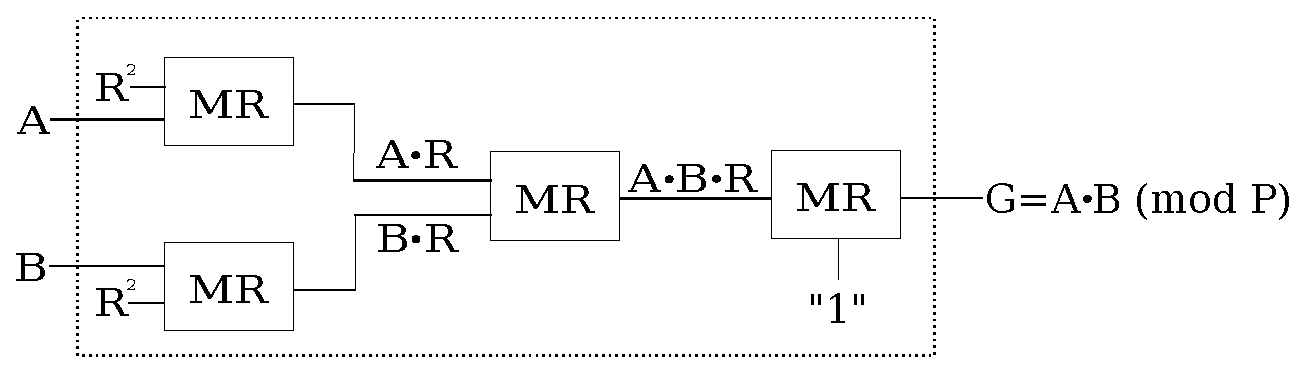
\includegraphics[scale=0.34]{new_mmcircuit}
  \caption{Montgomery multiplication.}
  \label{montfig}
  \end{figure}



\par Table~\ref{montmmsyn} provides the results for GBR on flattened
(bit-blasted) and  optimized Montgomery multipliers for the sequential
and parallel executions of Algorithm
\ref{multimon}. \textcolor{red}{The maximum  
memory consumption for sequential execution varies from 
66.7 MB for 64-bit operands to 11.3 GB for 571-bit operands.} 
% For most of these benchmarks the overhead is quite small than the
% reduction time for one bit except for the 233 and 409 bit
% multipliers. Therefore, we benefit from parallelizing the reduction
% process for these cases other than 283 and 409 bit multipliers.  
Our approach outperforms conventional explicit approaches except for
the case of 283 bit multiplier. 
% \textcolor{red}{Also, the reduction time for
% 283-bit circuit is more than 409-bit circuit. The reason is that 
% the bit-width of the multipliers is not the only factor controlling 
% the GBR time. The irreducible polynomial $P(x)$ also plays an
% important role in the designing of the multiplier and 
% consequently in the reduction as explained in \cite{cunxi:aspdac17}.} 

%%%%%%%%%%%%% Syn Mont Multipliers %%%%%%%%%%%%%%%%%%
%\iffalse
\begin{table}[H]
\centering
%\caption{Synthesized Mastrovito Multipliers (Time in seconds, \# of nodes, \# of redundant monomials in $k$)  (K = $10^3$, M = $10^6$)}
\caption{Montgomery Multipliers (Time in seconds); $k$ = Datapath Size, \#Gates = No. of gates, \#T = No. of threads, Time-Out = 30 hrs, (P): Parallel Execution, (S): Sequential Execution, K = $10^3$, M = $10^6$, PB: PolyBori, ZR: Algorithm~\ref{multimon}}
\label{montmmsyn}
\begin{tabular}{| c | c || c | c | c | c | c | c | c |} \hline
%\multirow{2}{*}{\textbf{Input}} & \multirow{2}{*}{\textbf{Abstraction}} & \multicolumn{3}{ c |}{\textbf{ZBDD reduction(ZR)}}  &  \multirow{2}{*}{\textbf{ZR improved}}\\ \cline{3-5}
% & &Building ZBDDs&Reduction&Total&\\ \hline
\multirow{2}{*}{$\boldsymbol{k}$}&\multirow{2}{*}{\textbf{\#Gates}}&\multirow{2}{*}{\textbf{F4~\cite{pruss:tcad}}}& \multirow{2}{*}{\textbf{\#T}}&\multirow{2}{*}{\textbf{~\cite{cunxi:aspdac17}(P)}}& \multicolumn{2}{ c |}{\textbf{PB}}&\multicolumn{2}{ c |}{\textbf{ZR}}\\ \cline{6-9}
&&&&&\textbf{(P)}&\textbf{(S)}&\textbf{(P)}&\textbf{(S)} \\ \hline
64 &9.5K&16.29&20&10.69&6.27&9.22& \textbf{3.75} & 8.37\\ \hline 
%96 &20.3K&&20&36.40&24.22& 22.0&\textbf{17.56} & 21.15\\ \hline 
128 &35K&621.90&20& 36.19&28.93&34.59&  \textbf{13.76}&24.73\\ \hline 
163 &56.5K&2,608.4&20&204.94 &167.73&335.2&  \textbf{141.68}&321.60\\ \hline 
233 &111K&385.92& 20&132.51& 119.77&99.36 &42.16&\textbf{31.88}\\ \hline
283 &165K&5,344& 20&\textbf{704.13}&1,194.2&2,078& 1,065.3&2,113\\ \hline
409 &340K&7,104& 10& 697.91&737.23& 722.1&303.91&\textbf{299.92}\\ \hline
571* &1.97M&TO&3&TO&CR&CR&\textbf{43,813}&99,042 \\ \hline
\end{tabular}
\end{table}
%\fi
%%%%%%%%%%%%%%%%%%%%%%%%%%%%%%%%%%%%%%%%%

\par Table \ref{montblockmm} presents the
statistics for Montgomery multipliers where the hierarchy of
Fig. \ref{montfig} for the blocks A, B, C, and D is made
available. The experiment first reduces the outputs of each individual
block modulo the gates of that block, and then reduces the primary
outputs modulo these four sets of remainders (ZBDDs), thus exploiting
the hierarchy of these circuits. Table~\ref{montblockmm} shows the time
for reduction of each block and the time for reducing the primary
outputs across the four blocks. The  time for reducing the primary
outputs across the hierarchical blocks in case of the F4
implementation is $<$1 second, and is not explicitly mentioned in the
table. The row labeled \textit{Total} presents the sum of the
computation time of 
reduction across these levels, and the maximum of the time to reduce
each MR block (as the reductions for the four blocks are independent
of each other and are parallelized). These results again demonstrate
the efficiency of our approach against explicit approaches.
% The datapath sizes of these circuits correspond to
% NIST-specification in cryptography with $k = 163,\dots,571$ bits.

\begin{table}[H]
\centering
% \caption{Montgomery Blocks(Time in seconds, Red. = time for reduction,
%   Coll. = time to reduce across the 4 levels.)}
\caption{Montgomery Blocks (Time in seconds); $k$ = Datapath Size, \#Gates = No. of gates, Time-Out = 30 hrs, 
Red. = time for reduction, Coll. = time to reduce across the 4 levels. 
% (P): Parallel Execution, (S): Sequential Execution, 
K = $10^3$, M = $10^6$, PB: PolyBori, ZR: Algorithm~\ref{multimon}}

\label{montblockmm}
\begin{tabular}{| c | c | c || c | c | c | c | c |} \hline
\multirow{2}{*}{$\boldsymbol{k}$}& \multirow{2}{*}{\textbf{\#Gates}}&\multirow{2}{*}{\textbf{Block}}& \multirow{2}{*}{\textbf{F4~\cite{pruss:tcad}}}  & \multicolumn{2}{ c |}{\textbf{PB}} &  \multicolumn{2}{ c |}{\textbf{ZR}} \\ \cline{5-8}
  & & & &Red. & Coll.  &Red. & Coll.  \\ \hline
\multirow{4}{*}{163} &33K &Block A & 25& 12 &\multirow{4}{*}{16} & 1 & \multirow{4}{*}{18}\\  \cline{2-5} \cline{7-7}
 & 33K&Block B &25 & 12 & & 1  &  \\  \cline{2-5} \cline{7-7}
 &85K&Block C &73 & 18 &&  7 &  \\  \cline{2-5} \cline{7-7}
 &32K&Block D &24 & 12 & & 1 & \\ \cline{2-8}
 &\multicolumn{2}{ c ||}{\textbf{Total}} & 73  &   \multicolumn{2}{ c |}{34} & \multicolumn{2}{ c |}{\textbf{25}}\\ \noalign{\hrule height 1.5pt}
\multirow{4}{*}{233}&55K&Block A  &142  & 32 & \multirow{4}{*}{5} & 0.14 & \multirow{4}{*}{4}\\  \cline{2-5} \cline{7-7}
 &55K& Block B &141 & 33 && 0.14  &  \\  \cline{2-5} \cline{7-7}
 &163K&Block C &408 & 34 & & 2.1  &  \\  \cline{2-5} \cline{7-7}
 &54K&Block D & 140& 32 && 0.13 & \\ \cline{2-8}
&\multicolumn{2}{ c ||}{\textbf{Total}}& 408  &   \multicolumn{2}{ c |}{39} & \multicolumn{2}{ c |}{\textbf{6.1}}\\ \noalign{\hrule height 1.5pt}
\multirow{4}{*}{283}&82K&Block A & 330 & 79 & \multirow{4}{*}{26} &24 & \multirow{4}{*}{90}\\  \cline{2-5} \cline{7-7}
&82K & Block B &329 & 78 && 23  &  \\  \cline{2-5} \cline{7-7}
&241K &Block C &883 & 173 &&  118 &  \\  \cline{2-5} \cline{7-7}
&81K &Block D &321 & 80 && 23 & \\ \cline{2-8}
&\multicolumn{2}{ c ||}{\textbf{Total}} & 883  &   \multicolumn{2}{ c |}{\textbf{199}} & \multicolumn{2}{ c |}{208}\\ \noalign{\hrule height 1.5pt}
\multirow{4}{*}{409}&168K&Block A & 1,322 & 177&\multirow{4}{*}{28} & 0.57 & \multirow{4}{*}{29}\\ \cline{2-5} \cline{7-7}
& 168K& Block B &1,335 &  175 &&  0.57 &  \\ \cline{2-5} \cline{7-7}
& 502K&Block C &4,471 & 192 &&  14 &  \\  \cline{2-5} \cline{7-7}
&168K &Block D &1,338 & 176 && 0.56 & \\ \cline{2-8}
&\multicolumn{2}{ c ||}{\textbf{Total}} & 4,471  &   \multicolumn{2}{ c |}{220} & \multicolumn{2}{ c |}{\textbf{43}}\\ \noalign{\hrule height 1.5pt}
\multirow{4}{*}{571}&330K&Block A &5,371 & 769 & \multirow{4}{*}{1,341} &321  & \multirow{4}{*}{1,412}\\  \cline{2-5} \cline{7-7}
&330K & Block B &5,421 & 747 && 332  &  \\ \cline{2-5} \cline{7-7}
 &980K&Block C &37,804 & 3,605 &&  3026 &  \\  \cline{2-5} \cline{7-7}
 &328K&Block D &5,539 & 751 && 338 & \\ \cline{2-8}
&\multicolumn{2}{ c ||}{\textbf{Total}}& 37,804  &   \multicolumn{2}{ c |}{4,946} & \multicolumn{2}{ c |}{\textbf{4,438}}\\ \noalign{\hrule height 1.5pt}


\end{tabular}
\end{table}


{\bf Equivalence Checking:} As a result of the GBR
$z_i\xrightarrow{G}_+ r_i$, the function implemented by each output
bit $z_i$ of the circuit is represented as a reduced, canonical,
Boolean polynomial in terms of the primary inputs, and by using a ZBDD.
Thus the equivalence of such vastly different arithmetic circuit
implementations (Mastrovito vs Montgomery) can be verified by testing
for the equality (isomorphism) of the corresponding ZBDD graphs. 


 %%%%%%%%% Point Addition Block D%%%%%%%%%%%%%%%%%%%%%%%%
\subsection{Point Addition over Elliptic Curves}
Point addition is an important operation required for the task of encryption, decryption 
and authentication in Elliptic Curve Cryptography (ECC). 
Modern approaches represent the points in projective
coordinate systems, {\it e.g.}, the L$\acute{o}$pez-Dahab (LD) projective coordinate \cite{eccld}, due to which the point addition 
operation can be implemented as polynomials in the field. 

\begin{Example}
{\it Consider point addition in L$\acute{o}$pez-Dahab (LD) projective coordinate. Given an elliptic curve: $Y^2 + XYZ = X^3Z + aX^2Z^2 + bZ^4$ over $\mathbb{F}_{2^k}$, where $X,Y,Z$ are $k$-bit vectors that are elements in $\mathbb{F}_{2^k}$ and similarly, $a, b$ are constants from the field. We represent point addition over the elliptic curve as ($X_3$, $Y_3$, $Z_3$) = ($X_1$, $Y_1$, $Z_1$) + ($X_2$, $Y_2$, $1$).  Then $X_3$, $Y_3$, $Z_3$ can be computed as follows:} 

\begin{align*}
&A = Y_2 \cdot Z_1^2 + Y_1  &&B = X_2 \cdot Z_1 + X_1 \\
&C = Z_1 \cdot B  &&D = B^2 \cdot(C + a Z_1^2) \\
&Z_3 = C^2 && E = A \cdot C  \\
&X_3 = A^2 + D + E &&F = X_3 + X_2 \cdot Z_3 \\
&G = X_3 + Y_2\cdot Z_3 && Y_3 = E\cdot F + Z_3 \cdot G \\
\end{align*}
\end{Example}

Each of the polynomials in the above design are implemented as a
(gate-level) logic block and are interconnected to obtain final
outputs $X_3,Y_3$ and $Z_3$. 

\begin{table}[H]
\centering
\caption{Point Addition Circuits (Time in seconds); $k$ = Datapath Size, \#Gates = No. of gates, Time-Out = 30 hrs, K = $10^3$, M = $10^6$,
PB: PolyBori, ZR: Algorithm~\ref{multimon}}
\label{pointadd}
\begin{tabular}{| c | c || c | c | c |} \hline
$\boldsymbol{k}$&\textbf{\#Gates}&\textbf{F4~\cite{pruss:tcad}}&\textbf{PB}&\textbf{ZR} \\ \hline
64&15.3K&1.78&3.32&\textbf{0.72} \\ \hline
128&64K&40.55&27.41&\textbf{6.03} \\ \hline
163&104K&130.24&57.57&\textbf{13.13} \\ \hline
233&139K&335.60&106.85&\textbf{19.62} \\ \hline
283&281K&1,787.96&273.53& \textbf{64.48}\\ \hline
409&423K&5,077.50&578.15& \textbf{115.20}\\ \hline
571&1.14M&48,162.29&CR&\textbf{725.95} \\ \hline
\end{tabular}
\end{table}

The word-level abstraction approach in~\cite{pruss:tcad} presents the
results for extracting  the above representation for each of
$A,B,\dots, X_3,Y_3,Z_3$ blocks. It first performs a bit-level
reduction for every output of each block (GBR $z_i\xrightarrow{G}_+
r_i$), and then a  bit-to-word substitution to derive an input-output
word-level representation for the circuit. Table~\ref{pointadd} shows
the comparison of the time required for bit-level reduction of outputs
$d_i$ of the block $D= B^2\cdot(C + aZ_1^2)$ as done
in~\cite{pruss:tcad} against our implementation. (Bit-level
reductions for other blocks take much less time than that for block
D.) This result demonstrates that our bit-level GBR implementation
is in many cases orders of magnitude faster than the F4-style
reduction of \cite{pruss:tcad}. Therefore our approach can replace the
F4-style bit-level GBR of \cite{pruss:tcad} and improve the overall
process of word-level abstraction of datapath designs.   

\subsection{Equivalence Checking of Sequential Galois Field Multipliers}
The designs discussed so far are combinational implementations of
polynomial computations of finite filed circuits. These designs use
the standard basis representation $\{1,\alpha,\alpha^2, \dots,
\alpha^{k-1}\}$ to model a $k$-bit data-word $Z$ in terms of its
constituent bits as $Z = z_0 + z_1 \alpha + z_2 \alpha^2 \cdots +
z_{k-1} \alpha^{k-1}$, with $\alpha$ being the primitive element for
that field $\mathbb{F}_{2^k}$. 

\par 
%The size of the multipliers presented in the above sections
%become prohibitively large as $k$ increases.  
There exists sequential
multipliers where $k$-bit inputs are loaded into $k$-bit registers,
and the $k$-bit result is available  after $k$ clock-cycle execution
of the machine. These multipliers use a {\it normal basis}
$\{\beta,\beta^{2},\beta^{4},\dots,\beta^{2^{k-1}}\}$ to  represent a
$k$-bit data-word $S$ in terms of its constituent bits as $S =
s_0\beta + s_1\beta^{2} + s_2\beta^{4} \cdots s_{k-1}\beta^{2^{k-1}}$,
with $\beta$ being the normal element. The relation between $\alpha$
and $\beta$ can be used to represent  the bits $z_i$ and $s_j$ in
terms of each other.  

% \par The Normal basis are more efficient when performing multiplication and 
% exponentiations. The exponentiation operation can be achieved by simple cyclic-shift of the input bits. 
% As multiplication is more complex than exponentiation, it is performed by constructing a binary-valued $\lambda$-matrix $M$.
% %and then performing $A\times M \times B^T$ for inputs $A$ and $B$. 
% If the  matrix $M$ satisfies the property that the number non-zero elements is $2k-1$ (for data-path size $k$), then the
% normal basis is called an optimal normal basis (ONB). ONB is desirable for the construction
% of finite field circuits.  

\par We perform equivalence checking between two different
architectures of {\it sequential multipliers with parallel output
  (SMPO)}, the Agnew-SMPO (AG-SMPO) by
G.B. Agnew~\cite{agnew1991implementation} and the RH-SMPO by
Reyhani-Masoleh and Hasan~\cite{RHmulti}. The values in the registers
for all intermediate states  in these multipliers are different
because they are based on two different mathematical principles.
However, the final state of the output registers (i.e. after $k$ clock
cycles) is the same as it is the result of the multiplication. In
order to perform equivalence checking, the circuits are unrolled
over $k$ time frames, and the GBR $s_i \xrightarrow{G}_+ r_i$ 
is performed to obtain a canonical $r_i$ ($G$ is the set of
polynomials for the unrolled circuit under RTTO). The ZBDDs for
respective $r_i$'s (for AG-SMPO and RH-SMPO) are compared to perform
equivalence check.    

% \par The authors in \cite{xiaojun:date15}\cite{xiaojun:phd} present an implicit unrolling approach for 
% sequential multipliers to derive a canonical word-level input-output relation. They present results for 
% two architectures of {\it sequential multipliers with parallel output (SMPO)} based on different 
% mathematical principles, the Agnew-SMPO (AG-SMPO) by G.B. Agnew~\cite{agnew1991implementation}
% and the RH-SMPO by Reyhani-Masoleh and Hasan~\cite{RHmulti}. 

%\par We perform the GBR $s_i \xrightarrow{G}_+ r_i$ for each output bit $s_i$ of the $k$-cycle unrolled 
% multipliers to obtain a canonical $r_i$. The $r_i$ can then be used to perform an equivalence check between the
% two architectures. 
Tables \ref{rhsmpo} and \ref{agsmpo} present the run-time of our
implementation for performing these reductions on RH-SMPO and AG-SMPO
architectures respectively, when compared with the approach presented
in \cite{pruss:tcad} and PolyBori. 
%Although normal bases exist for every $k$, optimal normal bases (ONB)
%do not. There are also different types of ONB. The values of $k$ in
%the tables correspond to Type-II ONB. For more details and a list of
%ONB field size, reader can refer to~\cite{gao:phd_normal_basis}. 
The results show that our implementation is about an order of
magnitude faster than PolyBori and multiple orders of magnitude faster
than the  explicit approach of~\cite{pruss:tcad}.
% The bit-widths in table are
% such that the corresponding normal basis are ONB. Our verification technique is multiple orders of magnitude faster than 
% that of~\cite{pruss:tcad} and an order of magnitude faster than the PolyBori.

\begin{table}[H]
\centering
\caption{RH-SMPO Multipliers \textcolor{red}{(Time in seconds)}; $k$ = Datapath Size, \#Gates = No. of gates, Time-Out = 30 hrs, K = $10^3$,
PB: PolyBori, ZR: Algorithm~\ref{multimon}}
\label{rhsmpo}
\begin{tabular}{| c | c | c | c | c | c | c | c | c |} \hline
$\boldsymbol{k=}$&65&81&89&131&173&233&281&410 \\ \hline
\textbf{\#Gates} & 13.6K&21.4K & 25.9K& 55.9K &96.5K&177K&258K&546K\\ \hhline{|=|=|=|=|=|=|=|=|=|}
\textbf{F4\cite{pruss:tcad}} &9.02 &26.65 & 42.46&294.7&874.3&3,404&7,328&23,610 \\ \hline
% \textbf{F4\cite{pruss:tcad}}   & 8.56&22.2 & 37.1&259.5&838.5&3,009&7566&23,610 \\ \hline %with bogus primitive polynomial
\textbf{PB}  &3.65 &6.07 & 7.42&28.22 &47.16&116.63&199.32&637.69\\ \hline
\textbf{ZR}  & \textbf{0.42}& \textbf{0.80}&\textbf{1.01} & \textbf{3.03}&\textbf{3.53}&
\textbf{8.12}&\textbf{13.27}&\textbf{52.09}\\ \hline
\end{tabular}
\end{table}

\begin{table}[H]
\centering
\caption{AG-SMPO Multipliers \textcolor{red}{(Time in seconds)}; $k$ = Datapath Size, \#Gates = No. of gates, Time-Out = 30 hrs, K = $10^3$,
PB: PolyBori, ZR: Algorithm~\ref{multimon}}
\label{agsmpo}
\begin{tabular}{| c | c | c | c | c | c | c | c | c |} \hline
$\boldsymbol{k=}$&65&81&89&131&173&233&281&410 \\ \hline
\textbf{\#Gates} &12.5K & 19.5K&23.6K&51.2K&89.4K&162K&236K&503K \\ \hhline{|=|=|=|=|=|=|=|=|=|}
\textbf{F4\cite{pruss:tcad}} &8.34 &20.46 &33.2&221.4&754.1&2,655&5,569&21,938\\ \hline
% \textbf{F4\cite{pruss:tcad}}  & 8.15& 19.18&29.1 &200.9&665.7&2,387&6,516&21,938 \\ \hline %with bogus primitive polynomial
\textbf{PB} &3.11 & 6.82& 9.21& 20.15&44.37&107.12&187.77&578.61\\ \hline
\textbf{ZR} &\textbf{0.44} &\textbf{0.77} &\textbf{0.91}& \textbf{2.51}&\textbf{3.39}&
\textbf{7.8}&\textbf{12.63}&\textbf{43.78}\\ \hline
\end{tabular}
\end{table}

% \begin{table}[H]
% \centering
% \caption{RH-SMPO Multipliers; $k$ = Datapath Size, \#Gates = No. of gates, Time-Out = 30 hrs, K = $10^3$,
% PB: PolyBori, ZR: Algorithm~\ref{multimon}}
% \label{rhsmpo}
% \begin{tabular}{| c | c | c | c | c | c | c | c | c | c | c |} \hline
% $\boldsymbol{k}$&33&51&65&81&89&131&173&233&281&410 \\ \hline
% \#Gates & 3.5K&8.5K & 13.6K&21.4K & 25.9K& 55.9K &96.5K&177K&258K&546K\\ \hhline{|=|=|=|=|=|=|=|=|=|=|=|}
% \cite{pruss:tcad} & 0.56& 3.3&9.02 &26.65 & 42.46&294.7&874.3&3,404&7,328& \\ \hline
% \cite{pruss:tcad} &0.88 &3.3 & 8.56&22.2 & 37.1&259.5&838.5&3,009&7566&23,610 \\ \hline %with bogus primitive polynomial
% PB &0.58 &1.96 &3.65 &6.07 & 7.42&28.22 &47.16&116.63&199.32&637.69\\ \hline
% ZR &\textbf{0.10} & \textbf{0.28}& \textbf{0.42}& \textbf{0.80}&\textbf{1.01} & \textbf{3.03}&\textbf{3.53}&
% \textbf{8.12}&\textbf{13.27}&\textbf{52.09}\\ \hline
% \end{tabular}
% \end{table}

% \begin{table}[H]
% \centering
% \caption{AG-SMPO Multipliers; $k$ = Datapath Size, \#Gates = No. of gates, Time-Out = 30 hrs, K = $10^3$,
% PB: PolyBori, ZR: Algorithm~\ref{multimon}}
% \label{agsmpo}
% \begin{tabular}{| c | c | c | c | c | c | c | c | c | c | c |} \hline
% $\boldsymbol{k}$&33&51&65&81&89&131&173&233&281&410 \\ \hline
% \#Gates &3.2K&7.7K&12.5K & 19.5K&23.6K&51.2K&89.4K&162K&236K&503K \\ \hhline{|=|=|=|=|=|=|=|=|=|=|=|}
% \cite{pruss:tcad} & 0.48& 2.78&8.34 &20.46 &33.2&221.4&754.1&2,655&5,569&\\ \hline
% \cite{pruss:tcad} &0.48 &2.76 & 8.15& 19.18&29.1 &200.9&665.7&2,387&6,516&21,938 \\ \hline %with bogus primitive polynomial
% PB & 0.52& 1.74&3.11 & 6.82& 9.21& 20.15&44.37&107.12&187.77&578.61\\ \hline
% ZR & \textbf{0.07}&\textbf{0.24} &\textbf{0.44} &\textbf{0.77} &\textbf{0.91}& \textbf{2.51}&\textbf{3.39}&
% \textbf{7.8}&\textbf{12.63}&\textbf{43.78}\\ \hline
% \end{tabular}
% \end{table}

% \begin{Example}
% {\it Consider a 3-bit RH-SMPO multiplier with output bits $\{r_2,r_1,r_0\}$ and input bits $\{p_2,p_1,p_0\}\{q_2,q_1,q_0\}$. 
% The multiplier performs the operation $R=P\cdot Q$, where $R=r_0\cdot \beta + r_1\cdot \beta^2 + r_2\cdot \beta^4$, 
% $P=p_0\cdot \beta + p_1\cdot \beta^2 + p_2\cdot \beta^4$ and $Q=q_0\cdot \beta +q_1\cdot \beta^2 + q_2\cdot \beta^4$. 
% Also consider a Mastrovito multiplier performing the operation $Z=A\cdot B$ with $Z=z_0\cdot  + z_1 \alpha + z_2\cdot \alpha^2$,
%  $A=a_0\cdot  + a_1 \alpha + a_2\cdot \alpha^2$ and $B=b_0  + b_1\cdot \alpha + b_2\cdot \alpha^2$ where $\{z_2,z_1,z_0\}$ and 
%  $\{a_2,a_1,a_0,b_2,b_1,b_0\}$ being the output and input bits respectively. The normal element $\beta$ in terms of standard basis 
%  element is $\beta = \alpha^3$. The primitive polynomial used in the design of Mastrovito multiplier is $P=X^3+X+1$ and $\alpha$ is the 
%  root of this polynomial.
%  \par The RH-SMPO multiplier output $R$ can be written in the notations of standard basis 
%  as $R = r_0\cdot \alpha^3 + r_1\cdot \alpha^6 + r_2\cdot \alpha^{12} = (r_0 + r_1 + r_2) + (r_0 + r_2)\cdot \alpha + (r_1 + r_2)\cdot \alpha^2$ using $\beta = \alpha^3$ and $\alpha^3 = \alpha +1$. Similarly, $P = (p_0 + p_1 + p_2) + (p_0 + p_2)\cdot \alpha + (p_1 + p_2)\cdot \alpha^2$ and $Q = (q_0 + q_1 + q_2) + (q_0 + q_2)\cdot \alpha + (q_1 + q_2)\cdot \alpha^2$. Therefore, }
% \begin{align*}
% & z_0 = r_0 + r_1 + r_2; ~~ z_1 = r_0 + r_2; ~~ z_2 = r_1 + r_2; \\
% & a_0 = p_0 + p_1 + p_2; ~~ a_1 = p_0 + p_2; ~~ a_2 = p_1 + p_2; \\
% & b_0 = q_0 + q_1 + q_2; ~~ b_1 = q_0 + q_2; ~~ b_2 = q_1 + q_2;
% \end{align*}
% {\it Solving for $p_i$ and $q_i$ in terms of $a_i$ and $b_i$ respectively,}
% \begin{align*}
% & p_0 = a_0 + a_2; ~~ p_1 = a_0 + a_1; ~~ p_2 = a_0 + a_1 + a_2; \\
% & q_0 = b_0 + b_2; ~~ q_1 = b_0 + b_1; ~~ q_2 = b_0 + b_1 + b_2;
% \end{align*}
% {\it Performing a bit-level reduction on $r_0,r_1$ and $r_2$ results in the following remainders,}
% \begin{align*}
% & r_0 = p_1\cdot q_0 + p_0\cdot q_1 + p_2\cdot q_1 + p_1\cdot q_2 + p_2\cdot q_2 \\
% & r_1 = p_0\cdot q_0 + p_2\cdot q_0 + p_2\cdot q_1 + p_0\cdot q_2 + p_1\cdot q_2 \\
% & r_2 = p_1\cdot q_0 + p_2\cdot q_0 + p_0\cdot q_1 + p_1\cdot q_1 + p_0\cdot q_2
% \end{align*}
% {\it Using $z_0 = r_0 + r_1 + r_2$, we get $z_0 = p_0\cdot q_0 + p_1\cdot q_1 + p_2\cdot q_2$. 
% Substituting $\{p_i,q_i\}$ in terms of $\{a_i,b_i\}$ results in $z_0 = a_0\cdot b_0 + a_1\cdot b_2 + a_2\cdot b_1$,
% which is also the remainder if we reduce the $z_0$ bit of the Mastrovito multiplier 
% modulo the polynomials of the gates of the circuit.
% }

% \end{Example}

% \begin{table}[H]
% \centering
% \caption{RH-SMPO Multipliers; k = Datapath Size, \#Gates = No. of gates, Time-Out = 30 hrs, K = $10^3$}
% \label{rhsmpo}
% \begin{tabular}{| c | c | c | c | c | c | c |} \hline
% \textbf{k}&33&51&65&81&89&99 \\ \hline
% \#Gates & 3.5K&8.5K & 13.6K&21.4K & 25.9K& 32K\\ \hline
% \cite{xiaojun:date15} & 112.6& 1,129&5,243 &20,724 &36,096 &67,021 \\ \hline
% PB & 0.59& 2.02&3.10 &5.99 &7.72 &13.26 \\ \hline
% ZR &\textbf{0.10} & \textbf{0.26}& \textbf{0.48}& \textbf{0.84}&\textbf{1.08} & \textbf{1.48}\\ \hline
% \end{tabular}
% \end{table}

% \begin{table}[H]
% \centering
% \caption{AG-SMPO Multipliers; k = Datapath Size, \#Gates = No. of gates, Time-Out = 30 hrs, K = $10^3$}
% \label{agsmpo}
% \begin{tabular}{| c | c | c | c | c | c |} \hline
% \textbf{k}&36&66&82&89&100 \\ \hline
% \#Gates &3.8K&13K&20K & 23.6K&29.8K \\ \hline
% \cite{xiaojun:date15} & 113& 3,673& 15,117& 28,986& 50,692\\ \hline
% PB &0.48 & 2.84& 6.93&7.29 & 9.91 \\ \hline
% ZR & \textbf{0.10}&\textbf{0.46} &\textbf{0.76} &\textbf{0.95} &\textbf{1.30} \\ \hline
% \end{tabular}
% \end{table}


\subsection{Limitations of our approach: Integer arithmetic circuits}
% \par {\bf Integer Multiplication:} When performing reduction on
% integer multiplication benchmarks, a large number of non-linear  %
% monomials are generated that can be canceled early in the reduction
% process by employing a word-level approach unlike  % our bit-level
% reduction approach.  % The polynomial algebra model is not suitable
% for random logic (synthesized) circuits, where AIG-based reduction
% makes verification efficient. This model is beneficial for custom
% designed arithmetic circuits, where AIGs/SAT fail. 
\textcolor{red}{
The GBR approach presented in the previous section, although
applicable to integer arithmetic circuits, is not computationally
feasible for their verification. 
%The logical cones of output variables in integer
%arithmetic circuits have a lot of logic sharing (common subexpressions) and generate a
%large number of non-linear terms. 
We evaluated  our technique on integer arithmetic multiplier
circuits, which showed an  exponential increase in verification time
$w.r.t.$ the circuit size. This is because our approach reduces 
each primary output bit independently, and does not consider the logic
sharing among different primary outputs. As a result, a large number
of monomials are generated during reduction that are common to 
multiple primary outputs. This effect of logic sharing cannot be
exploited in GBR when each primary output bit is reduced
independently. 
For example, the ZBDD-based bit-level GBR for a 7x7 integer
multiplier reveals that when reducing the $z_{13}$ bit (MSB) and
the $z_{12}$ bit independently, the maximum number of monomials
encountered ($i.e.$ during $z_{13} \xrightarrow{G}_+ r_{13}$ and
$z_{12} \xrightarrow{G}_+ r_{12}$) are 429,889 and 897,955,
respectively.  However, the modulo-2 sum (XOR) of these ZBDDs contains
only 789,604 monomials  (during the modulo-2 sum common monomials
cancel out) as opposed to 1,327,844 (= 429,889 + 897,955).
A word-level reduction approach (such as those of
\cite{ciesielski:dac2015} and \cite{rolf:date16}) may cancel such
common non-linear terms early in the reduction process and avoid
intermediate blow-up in the number of monomials. This is shown below.
%This  
%implies that even an implicit data-structure
%cannot accommodate the large number of non-linear terms
%that result in intermediate expression swell.
% Performing a detailed analysis reveals that for
% integer arithmetic datapath circuits, a bit-level reduction is {\it
%   not sufficient} for verification efficiency, and a word-level
% approach is required. %, such as the ones presented in 
}

\begin{figure}[hbt]
\centering
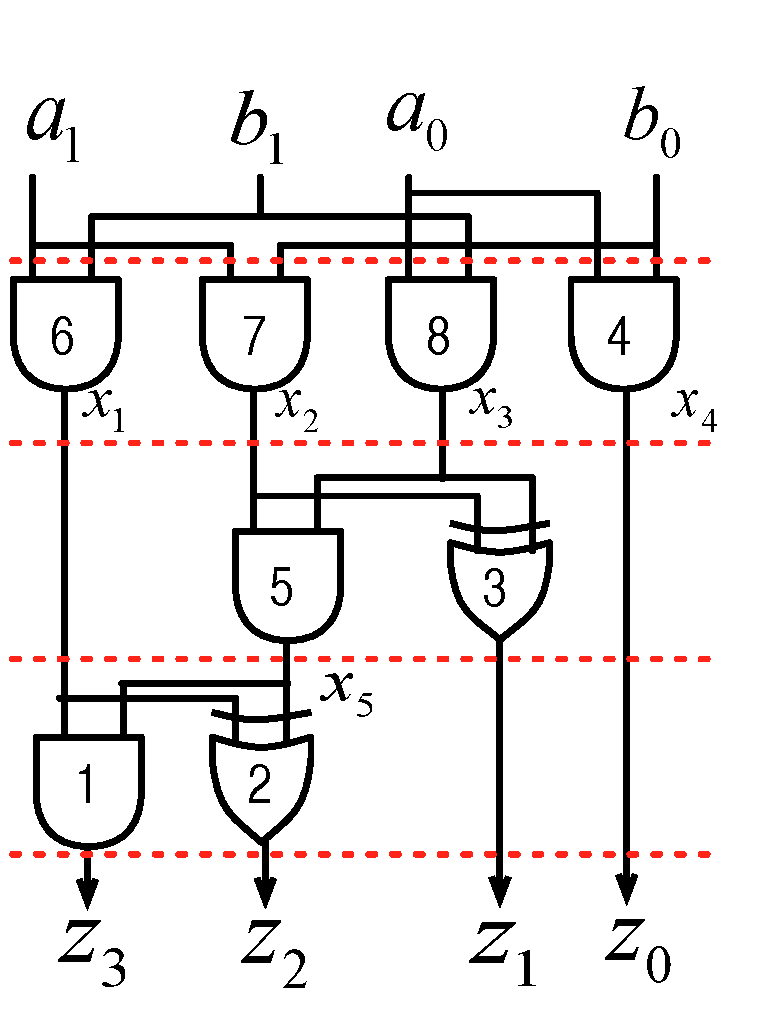
\includegraphics[scale=0.4]{2-bit-mult.pdf}
\caption{Integer multiplier circuit}
\label{intmult}
\end{figure}

%\textcolor{red}{ A better 
%approach would be to perform a word-level reduction similar to
%the following example.
%}

\textcolor{red}{Consider the integer multiplier circuit given in
  Fig. \ref{intmult}. A 
word-level approach would model the output word as 
$Z = z_0 + 2z_1 + 4 z_2 + 8 z_3$, and perform the reduction
$Z\xrightarrow{G}_+R$ across the reverse topological levels (RTTO) 
depicted in the figure. The polynomials of the circuit are:} 

\textcolor{red}{\begin{align*}
z_0 &= x_4\\
z_1 &= x_2 + x_3 - 2x_2x_3\\
z_2 &= x_1 + x_5 - 2 x_1 x_5\\
    &= x_1 + x_2x_3 - 2x_1x_2x_3\\
z_3 &= x_1x_5 = x_1x_2x_3
\end{align*}}

\textcolor{red}{Here $+$ denotes addition over integers. The reduction
  of the word-level expression $8z_3 + 4z_2+2z_1+z_0$ in $Z$ cancels out the
  common nonlinear monomials to control intermediate monomial explosion: }

\textcolor{red}{\begin{align*}
Z &= 8z_3 + 4z_2+2z_1+z_0\\
  &=\underline{8x_1x_2x_3} + (4x_1 + \underbrace{4x_2x_3} -
  \underline{8x_1x_2x_3})\\
  & + (2x_2+2x_3-\underbrace{4x_2x_3}_{}) + x_4\\
  &=\textcolor{red}{4x_1 + 2x_2 + 2x_3 + x_4}
\end{align*}
}

\textcolor{red}{A purely
bit-level GBR approach is thus not suitable for integer arithmetic
circuits. However, this is not a limitation of our algorithms and
implementations, but rather an issue of the capability of bit-level
versus word-level models. Integrating the implicit data structure with
a word-level representation may yield better results for
such applications.} 

%% This modulo-2 sum indicates that reducing all the outputs simultaneously results 
%% in monomials that can cancel each other. Therefore, verification of integer multipliers require a word-level
%% decision procedure, as given in \cite{ciesielski:dac2015}
%% \cite{rolf:date16}, that accounts for the cancellation of these
%% monomials across multiple bits in one word-level expression whereas a pure bit-level reduction
%% is not sufficient to solve the problem. The experiment suggests that for integer 
%% arithmetic multipliers, 



% The reduction times for small integer arithmetic array multipliers are
% presented in Table \ref{intmm}. There is an 8x increase in time when
% moving from $n-1$ datapath size to $n$-bits, which is an exponential
% increase. Performing detailed analysis of a 7x7 multiplier reveals
% that, when reducing the $z_{13}$ bit (MSB) and $z_{12}$ bit of this
% circuit, the maximum number of monomials encountered are 429,889 and
% 897,955. Of these, 269,120 monomials are {\it common to both output
%   bits}. This implies that integer multipliers require a word-level
% decision procedure, as given in \cite{ciesielski:dac2015}
% \cite{rolf:date16}, that account for the cancellation of these
% monomials across multiple bits in one word-level expression. Our
% results show that bit-level techniques cannot efficiently verify
% integer arithmetic circuits, but are very efficient for finite-field
% arithmetic circuits. 

% \begin{table}[H]
% \centering
% \caption{Integer Array Multipliers (Time in seconds)}
% \label{intmm}
% \begin{tabular}{| c | c | c | c | c |} \hline
% \textbf{Datapath}&7&8&9&10 \\ \hline
% \textbf{Time}& 1& 8 &66&478 \\ \hline
% \end{tabular}
% \end{table}


%%%%%%%%%%%%%%%%%%%%%%%%%%%%%%%%%%%%%%%%%%%%%%%%%%%%%%%%

\section{Conclusion} \label{sec:conc}
This paper has presented an approach for formal verification of 
datapath circuits by deriving a canonical polynomial representation
for each output bit $z_i$ of a circuit in terms of the primary inputs
using Gr\"obner basis reduction. The gates of the circuit $C$ are
modeled as a set of polynomials $G$ over $\mathbb{F}_2$ where the
variables are the nets of the circuit. An order on the variables is
derived from the topology of the circuit, and a $lex$ term order
(RTTO) is imposed on the polynomials. RTTO renders the set $G$ a
Gr\"obner basis  itself. The reduction $z_i\xrightarrow{G}_+ r_i$
results in a canonical remainder $r_i$ for  each output $z_i$. 
%The complexity of computing the
%Gr\"obner basis can be avoided by deriving a term order from th
%topology of the circuit, which renders this set of polynomials itself
%as  a Gr\"obner basis. 
\par The polynomials in the set $G$ are Boolean polynomials that can 
be construed as unate cube sets. The unate cube set algebra prowess of
ZBDDs is exploited to represent the polynomials implicitly. We show
that RTTO imposes a special structure on the ZBDDs, where
subexpressions for leading monomials and quotients of the division are
readily visible as subgraphs in the ZBDD. We take further advantage of
this data structure to improve the classical \Grobner basis reduction 
method that relies on canceling only 1 monomial in every iteration
of division. Our approach cancels multiple monomials in each step of
division and generates fewer terms, thus speeding up the reduction. 
We have performed experiments with various finite field circuits used in
cryptography. Our approach achieves significant improvement over
recent approaches: the F4-style reduction, a parallelized approach for
reduction, and PolyBori. 
% The  efficiency of our approach is demonstrated by completing the
% reduction for up to 571-bit modulo Montgomery multipliers in the allotted time,
% and significant improvement is achieved over the F4-style reduction,
% parallelized reductions and  PolyBori based techniques. 

As part of our future work, we are pursuing investigations to
discover a pseudo-Boolean ``word-level signature'' of the GBR
$Z\xrightarrow{G}_+R$, that could be integrated with implicit
representations for integer arithmetic circuits.   

\par \textbf{Acknowledgment:} The authors wish to thank Cunxi Yu of
the University of Massachusetts, Amherst for assistance with
logic synthesis and optimization of some of the benchmarks used in the
experiments.  
%\end{document} 
%%%%%%%%% Mas571 Multipliers %%%%%%%%%%%%%%%%%%%%%%%%
\iffalse
\begin{table}[H]
\centering
\caption{Structured 571 bit Multipliers (Time in seconds);  \#Gates = No. of gates, \#T = No. of threads, Time-Out = 1 day, (P): Parallelization, (WP): Without Parallelization, K = $10^3$}
\label{montmmsyn}
\begin{tabular}{| c | c | c | c | c | c | c | c |} \hline
\textbf{Architecture} & \textbf{\#Gates}&\textbf{F4} & \textbf{\#T} & \textbf{~\cite{cunxi:aspdac17}(P)} & \textbf{PB} & \textbf{ZR(P)} & \textbf{ZR(WP)} \\ \hline
Mastrovito&1,600K&TO&3&5,331&CR&2,126.65&566 \\ \hline
Montgomery&1,970K&TO&3&TO&CR&43,813&TO \\ \hline
\end{tabular}
\end{table}
\fi
%%%%%%%%%%%%%%%%%%%%%%%%%%%%%%%%%%%%%%%%%
%%%%%%%%% OLD TABLES%%%%%%%%%%%%%%%%%%%%%%%%%%
%%%%%%%%%%%%%%%%%%%%%%%%%%%%%%%%%%%%%%%%%
%%%%%%%%%%%%%%%%%%%%%%%%%%%%%%%%%%%%%%%%%
\iffalse
\begin{table*}
\centering
\caption{Mastrovito Multipliers (Time in seconds, \# of nodes, \# of redundant monomials in $k$)  (K = $10^3$, M = $10^6$)}
\label{masmm}
\begin{tabular}{| c | c | c | c | c | c | c |} \hline
%\multirow{2}{*}{\textbf{Input}} & \multirow{2}{*}{\textbf{Abstraction}} & \multicolumn{3}{ c |}{\textbf{ZBDD reduction(ZR)}}  &  \multirow{2}{*}{\textbf{ZR improved}}\\ \cline{3-5}
% & &Building ZBDDs&Reduction&Total&\\ \hline
\textbf{Datapath(k)}&\textbf{\# of Gates} & \textbf{F4} & \textbf{PB} &\textbf{ZR} & \textbf{MN/MR} & \textbf{CS}\\ \hline
163 &153K& 1,443s &70s& \textbf{10s} & 811/765 & 153K\\ \hline 
233 &167K& 1,913s &105s& \textbf{14s} & 772/699& 167K\\ \hline
283 &399K& 11,116s &316s& \textbf{45s} & 1,413/1,402&400K\\ \hline
409 &508K& 17,848s &596s& \textbf{75s} & 1,313/1,227&508K\\ \hline
571 &1.6M& 192,032s &CR& \textbf{616s} & 2,849/2,840&1.6M\\ \hline 


\end{tabular}
\end{table*}
\fi

\iffalse
\begin{table*}
\centering
\caption{Montgomery Flat Multipliers (Time in seconds, \# of nodes in $k$, \# of redundant monomials in $k$) (K = $10^3$, M = $10^6$, B = $10^9$)}
\label{montmm}
\begin{tabular}{| c | c | c | c | c | c | c |} \hline
%\multirow{2}{*}{\textbf{Input Bit-width}} & \multirow{2}{*}{\textbf{Abstraction}} & \multicolumn{3}{ c |}{\textbf{ZBDD reduction(ZR)}}  &  \multirow{2}{*}{\textbf{ZR improved}} \\ \cline{3-5}
% & &Building ZBDDs&Reduction&Total& \\ \hline
\textbf{Datapath(k)}&\textbf{\# of Gates} & \textbf{F4} & \textbf{PB} &\textbf{ZR} & \textbf{MN/MR} & \textbf{CS}\\ \hline
163 & 184K&6,897s &\textbf{9294s}&9,595 & 39.4K/765 & 823M\\ \hline 
233 & 329K&63,805s &1749s&\textbf{1,452s}&4.4K/699 & 186M\\ \hline
283 & 488K&TO &\textbf{127,096s}& 247,837s &117K/1.4K &8.7B\\ \hline
409 & 1.0M&TO & \textbf{19,679s}& 32,226s &9.5K/1.2K &1.4B\\ \hline
571 & 1.97M&TO &CR& \textbf{128,464s}& TO/2.9K & TO\\ \hline 

\end{tabular}
\end{table*}
\fi

\iffalse
\begin{table*}
\centering
\caption{Montgomery Blocks(Max Nodes/Remainder)  (K = $10^3$, M = $10^6$)}
\label{montblockstats}
\begin{tabular}{| c | c | c | c | c | c | c |} \hline
\textbf{Datapath(k)/Block} &&  \textbf{163} & \textbf{233} &\textbf{283} & \textbf{409} & \textbf{571} \\ \hline
\multirow{2}{*}{Block A} &MN/MR&64/9&10/5&155/10&11/5& 296/9\\ \cline{2-7}
& CS&301K & 98K& 2.3M & 345K & 17M\\ \hline
\multirow{2}{*}{Block B} &MN/MR&64/9&10/5&155/10&11/5& 296/9\\ \cline{2-7}
& CS&301K & 98K& 2.3M & 345K & 17M\\ \hline
\multirow{2}{*}{Block C} &MN/MR&3.2K/3.2K&705/701&13K/10K&1.2K/1.2K& 83K/82K\\ \cline{2-7}
& CS&301K & 98K& 2.3M & 345K & 17M\\ \hline
\multirow{2}{*}{Block D} &MN/MR&112/58&12/7&292/147&14/8& 578/291\\ \cline{2-7}
& CS&301K & 98K& 2.3M & 345K & 17M\\ \hline
\multirow{2}{*}{Collapse} &MN/MR&18K/765&1.5K/699&42K/1.4K&3K/1.2K& 167K/2.8K\\ \cline{2-7}
& CS& 1.8M& 321K & 12M&1.3M &96M \\ \hline
\end{tabular}
\end{table*}
\fi
%&&&&&&&&&& \\ \hline
%%%%%%%%%%%%%%%%%%%%%%%%%%%%%%%%%%%%%%%%%
%%%%%%%%%OLD TABLES END%%%%%%%%%%%%%%%%%%%%%%%%
%%%%%%%%%%%%%%%%%%%%%%%%%%%%%%%%%%%%%%%%%
%%%%%%%%%%%%%%%%%%%%%%%%%%%%%%%%%%%%%%%%%




\iffalse
\begin{table}
\centering
\caption{Integer Array Multipliers (Time in seconds)}
\label{intmm}
\begin{tabular}{| c | c | c | c | c |} \hline
\textbf{Datapath}&7&8&9&10 \\ \hline
\textbf{Time}& 1& 8 &66&478 \\ \hline
\end{tabular}
\end{table}

\fi

%%%%%%%%%%%%%%%%%% ENDS HERE %%%%%%%%%%%%%%%%%
\iffalse

\begin{table}
\centering
\caption{Montgomery Blocks(Time in seconds)}
\begin{tabular}{| c | c | c | c | c | c | c | c | c | c | c | c | c | c | c | c | } \hline
\multirow{2}{*}{\textbf{Input/Blocks}} & \multicolumn{3}{ c |}{\textbf{163}} & \multicolumn{3}{ c |}{\textbf{233}} & \multicolumn{3}{ c |}{\textbf{283}} & \multicolumn{3}{ c |}{\textbf{409}} & \multicolumn{3}{ c |}{\textbf{571}} \\ \cline{2-11}
&ABS&PB&ZR&ABS&PB&ZR&ABS&PB&ZR&ABS&PB&ZR&ABS&PB&ZR  \\ \hline
Block A &25&1&142&$<1$&330&28&1,322&$<1$&5,371&725 &&&&&\\ \hline
Block B &25&1&141&$<1$&329&29&1,335&$<1$&5,421&752 &&&&&\\ \hline
Block C &73&12&408&13&883&254&4,471&117&37,804&4,164 &&&&&\\ \hline
Block D &24&1&140&$<1$&321&30&1,338&$<1$&5,539&747 &&&&&\\ \hline
Collapse &$<1$&33&$<1$&9&$<1$&158&$<1$&58&$<1$&1,516 &&&&&\\ \hline 
Total &&&&&&&&&& &&&&&\\ \hline
\end{tabular}
\end{table}
 \fi


%%%%%%%%%%%%%%%%%%%% The bibliography %%%%%%%%%%%%%%%%%%%%%%%%%%%%
\bibliographystyle{IEEEtran}
\bibliography{tim,xiaojun,utkarsh,logic,oldlogic}

\end{document}

%%%%%%%%%%%%%%%%%%%%%%%%%%%  End of IEEEsample.tex  %%%%%%%%%%%%%%%%%%%%%%%%%%%
